% This is LLNCS.DEM the demonstration file of
% the LaTeX macro package from Springer-Verlag
% for Lecture Notes in Computer Science,
% version 2.4 for LaTeX2e as of 16. April 2010
%
\documentclass{llncs}
%
\usepackage{makeidx}  % allows for indexgeneration
\usepackage{xspace}
\usepackage{comment}
\usepackage{mathpartir}
\usepackage{wrapfig}
\usepackage[inline]{enumitem}
\usepackage{bussproofs}
\usepackage{bussproofs}
\usepackage{dsfont}
\usepackage{xspace}
\usepackage{mathtools}
\usepackage{mathpartir}
\usepackage{listings}
\usepackage{color}
\usepackage{pifont}
\usepackage{amssymb}
\usepackage{moresize}
\usepackage[T1]{fontenc}
\usepackage[utf8]{inputenc}
\definecolor{pblue}{rgb}{0.13,0.13,1}
\definecolor{pgreen}{rgb}{0,0.5,0}
\definecolor{pred}{rgb}{0.9,0,0}
\definecolor{pgrey}{rgb}{0.9,0.9,0.91}
\definecolor{mygray}{rgb}{0.5,0.5,0.5}
\usepackage{listings}
\lstset{language=Java,
  showspaces=false,
  showtabs=false,
  breaklines=true,
  showstringspaces=false,
  breakatwhitespace=false,
  commentstyle=\color{pgreen},
  keywordstyle=\color{pblue},
  stringstyle=\color{pred},
  basicstyle=\fontsize{6.5}{7}\tt,
  tabsize=1,
  numbers=left,
  numbersep=2pt,
  numberstyle=\tiny\color{mygray},
  moredelim=[il][\textcolor{pgrey}]{$$},
  moredelim=[is][\textcolor{pgrey}]{\%\%}{\%\%}
}
\lstset{escapeinside={(*@}{@*)}}



%% Note: Authors migrating a paper from PACMPL format to traditional
%% SIGPLAN proceedings format should change 'acmlarge' to
%% 'sigplan,10pt'.

\usepackage{lipsum}  
%% Some recommended packages.
\usepackage{booktabs}   %% For formal tables:
                        %% http://ctan.org/pkg/booktabs
\usepackage{subcaption} %% For complex figures with subfigures/subcaptions
\captionsetup{compatibility=false}

%
\begin{document}
%
\frontmatter          % for the preliminaries
%
\newcommand{\tool}[0]{{\sc syncope}\xspace} % short for SYNthesizing
% COnsistency Property Enforcement.
\newcommand{\conj}{~\wedge~}

\newcommand{\HA}{{\sf HA}}
\newcommand{\SA}{{\sf SA}}
\newcommand{\UA}{{\sf UA}}
\newcommand{\scc}{\psi_{\sf sc}}
\newcommand{\ccc}{\psi_{\sf cc}}
\newcommand{\ecc}{\psi_{\sf ec}}
\newcommand{\rcc}{\psi_{\sf rc}}
\newcommand{\mavc}{\psi_{\sf mav}}
\newcommand{\rrc}{\psi_{\sf rr}}
%\newcommand{\coloneqq}{::=}
\newcommand{\spc}{\quad}

% \newtheorem{theorem}{Theorem}
% \newtheorem{lemma}[theorem]{Lemma}
% \newtheorem{proposition}[theorem]{Proposition}
% \newtheorem{corollary}[theorem]{Corollary}
% \newtheorem{definition}[theorem]{Definition}
% \newcounter{hno}
%   \newcounter{gno}
% \renewenvironment{proof}{\setcounter{hno}{0}\setcounter{gno}{0}
%   \emph{Proof.}}{}
% \newcommand{\npp}{\thehno \stepcounter{hno}}
% \newcommand{\mpp}{\thegno \stepcounter{gno}}

\newcommand{\stretcharraybig}{\renewcommand*{\arraystretch}{1.25}}
\newcommand{\cureff}{\hat{\eta}}
\newcommand{\eff}{\eta}
\newcommand{\fresh}{\N{\sf fresh}}
\newcommand{\cv}{\psi}
\newcommand{\ALT}{~\mid~}
\newcommand{\eid}{{\iota}}
\newcommand{\ObjType}{{\sf ObjType}}
\newcommand{\AbsType}{{\sf AbsType}}
\newcommand{\dom}{{\sf dom}}
\newcommand{\DtLib}[1]{\mathbb{D}(#1)}
\newcommand{\DtLibZ}{\mathbb{D}}
\newcommand{\Ops}{\Lambda}
\newcommand{\Ctrts}{\Psi}
\newcommand{\true}{\N{\textsf{true}}}

\newcommand{\R}[1]{\textrm{#1}}
\newcommand{\N}[1]{{\normalfont #1}}
\newcommand{\ObjZ}{\N{\textsf{Obj}}}
\newcommand{\Obj}[1]{\N{\textsf{Obj}_{#1}}}
\newcommand{\ReplID}{\mathtt{ReplID}}
\newcommand{\SessID}{\mathtt{SessID}}
\newcommand{\typeFun}[1]{\N{\textsf{type}}(#1)}
\newcommand{\Op}[1]{\N{\textsf{Op}_{#1}}}
\newcommand{\set}[1]{\mathcal{P}(#1)}
\newcommand{\unitVal}{\N{\textsf{unit}}}
\newcommand{\EffUniv}{\N{\sf Effect}}
\newcommand{\EffID}{\mathtt{SeqNo}}
\newcommand{\TransID}{\N{\sf TransID}}
\newcommand{\AVal}[1]{\N{\textsf{AVal}_{#1}}}
\newcommand{\RVal}[1]{\N{\textsf{RVal}_{#1}}}
\newcommand{\Eff}[1]{\N{\textsf{Eff}_{#1}}}
\newcommand{\loud}[1]{\textbf{\textit{#1}}}
\newcommand{\dt}[1]{\mathcal{D}_{#1}}
\newcommand{\vis}[2]{\N{\textsf{vis}(#1,#2)}}
\newcommand{\visZ}{\N{\textsf{vis}}}
\newcommand{\depsZ}{\N{\textsf{deps}}}
\newcommand{\deps}[1]{\N{\textsf{deps}(#1)}}
\newcommand{\Rvis}{\N{\textsf{vis}}}
\newcommand{\arZ}{\N{\textsf{ar}}}
\newcommand{\ar}[2]{\N{\textsf{ar}(#1,#2)}}
\newcommand{\stxZ}{\sim}
\newcommand{\stx}[2]{#1\sim#2}
\newcommand{\nstx}[2]{#1\not\sim#2}
\newcommand{\comZ}{\N{\textsf{com}}}
\newcommand{\com}[1]{\comZ(#1)}
\newcommand{\so}[2]{\N{\textsf{so}(#1,#2)}}
\newcommand{\soZ}{\N{\textsf{so}}}
\newcommand{\stZ}{\N{\textsf{st}}}
\newcommand{\Rso}{\N{\textsf{so}}}
\newcommand{\Rst}{\N{\textsf{st}}}
\newcommand{\COM}{\textrm{\sc {\small Commit}}}
\newcommand{\soo}[2]{\N{\textsf{soo}(#1,#2)}}
\newcommand{\sooZ}{\N{\textsf{soo}}}
\newcommand{\hb}[2]{\N{\textsf{hb}(#1,#2)}}
\newcommand{\hbo}[2]{\N{\textsf{hbo}(#1,#2)}}
\newcommand{\hbZ}{\N{\textsf{hb}}}
\newcommand{\hboZ}{\N{\textsf{hbo}}}
\newcommand{\txnZ}{\N{\textsf{txn}}}
\newcommand{\txn}[2]{\txnZ\{#1\}\{#2\}}
\newcommand{\sameobj}[2]{\N{\textsf{sameobj}(#1,#2)}}
\newcommand{\sameobjZ}{\N{\textsf{sameobj}}}
\newcommand{\sametxn}[2]{\N{\textsf{sametxn}(#1,#2)}}
\newcommand{\sametxnZ}{\N{\textsf{sametxn}}}
\newcommand{\E}{\N{\textsf{E}}}
\newcommand{\Pool}{\N{\textsf{pool}}}
\newcommand{\Cache}{\N{\textsf{cache}}}
\newcommand{\Avail}{\N{\textsf{avail}}}
\newcommand{\CacheFinder}{\N{\textsf{Ctxt}}}
\newcommand{\EffSoup}{\N{\textsf{A}}}
\newcommand{\obj}{\N{\textsf{obj}}}
\newcommand{\dep}{\N{\textsf{dep}}}
\newcommand{\ssn}{\N{\textsf{ssn}}}
\newcommand{\id}{\N{\textsf{id}}}
\newcommand{\oper}{\N{\textsf{oper}}}
\newcommand{\rval}{\N{\textsf{rval}}}
\newcommand{\repl}{\N{\textsf{repl}}}
\newcommand{\sess}{\N{\textsf{sess}}}
\newcommand{\rdtspec}{\Delta}
\newcommand{\goesto}{\longrightarrow}
\newcommand{\tuplee}[1]{\langle #1 \rangle}
\newcommand{\ctxtFn}{\N{\textsf{ctxt}}}
\newcommand{\rdtredsto}{\N{\leadsto}}
\newcommand{\Exec}{\N{\textsf{(\EffSoup,\allowbreak \visZ,\allowbreak \soZ)}}}
\newcommand{\pll}{~\|~}
\newcommand{\Mod}[1]{\N{\textsf{Mod}}(#1)}
\newcommand{\De}[1]{#1}
\newcommand{\Der}[2]{[\![#1,#2]\!]_{r}}
\newcommand{\msentails}[2]{#1 \models #2}
\newcommand{\hasTyp}[2]{#1 \vdash #2}
\newcommand{\auxred}[4]{#1 \vdash #2 \xhookrightarrow{#3} #4 }
\renewcommand{\qed}{\nobreak \ifvmode \relax \else
      \ifdim\lastskip<1.5em \hskip-\lastskip
      \hskip1.5em plus0em minus0.5em \fi \nobreak
      \vrule height0.75em width0.5em depth0.25em\fi}


% Operational semantics rules
\newcommand{\rulelabel}[1]{\textrm{\sc {\small [#1]}}}
\newcommand{\RULE}[3]
{\frac{\begin{array}{c}#1\end{array}}
		 {\begin{array}{c}#2\end{array}}
~ \rulelabel{#3}
}

\newcommand{\RuleTwo}[2]
{\frac{\begin{array}{c}#1\end{array}}
		 {\begin{array}{c}#2\end{array}}
}

\newenvironment{nop}{}{}
\newenvironment{smathpar}{
\begin{nop}\small\begin{mathpar}}{
\end{mathpar}\end{nop}\ignorespacesafterend}

\newenvironment{cmathpar}{
\vspace{-3mm}
\renewcommand{\arraystretch}{1.2}
\begin{nop}\begin{mathpar}}{
\end{mathpar}\end{nop}\ignorespacesafterend}

\newcommand{\rsf}[1]{\R{\sf #1}}
\newcommand{\trans}[4]{\N{\textsf{trans}}\{#1,#2\}\{#3,#4\}}

\setlength{\floatsep}{5pt}
\setlength{\textfloatsep}{10pt}
\setlength{\dblfloatsep}{5pt}
\setlength{\dbltextfloatsep}{10pt}


\newcommand{\ecds}{ECDS\xspace}
%\newcommand{\nexists}{\not\exists}
%\newcommand{\nsucc}{\not\succ}

%
\pagestyle{headings}  % switches on printing of running heads
\addtocmark{Hamiltonian Mechanic} % additional mark in the TOC
%
%
\mainmatter              % start of the contributions
%
\title{\tool : Automatic Enforcement of Distributed Consistency Guarantees}
%
\titlerunning{Hamiltonian Mechanics}  % abbreviated title (for running head)
%                                     also used for the TOC unless
%                                     \toctitle is used
%
\author{Kia Rahmani\inst{1} \and Gowtham Kaki\inst{1}\and Suresh
Jagannathan\inst{1}}
%
\authorrunning{Kia Rahmani et al.} % abbreviated author list (for running head)
%
%
\institute{Purdue University, West Lafayette IN 47906, USA\\
\email{\{rahmank,gkaki,suresh\}@purdue.edu}\\
%\texttt{http://users/\homedir iekeland/web/welcome.html}
}
\maketitle              % typeset the title of the contribution

\begin{abstract}

  Designing reliable and highly available distributed applications
  typically requires data to be replicated over geo-distributed
  stores.  But, such architectures force application developers to
  make an undesirable tradeoff between ease of reasoning, possible
  when replicated data is required to be strongly consistent, and
  performance, possible only when such guarantees are weakened.
  Unfortunately, undesirable behaviors may arise under weak
  consistency that can violate application correctness, forcing
  designers to either implement ad-hoc mechanisms to avoid these
  anomalies, or choose to run applications using stronger levels of
  consistency than necessary. The former approach introduces unwanted
  complexity, while the latter sacrifices performance.

  In this paper, we describe a lightweight runtime verification system
  that relieves developers from having to make such tradeoffs.
  Instead, our approach leverages declarative axiomatic specifications
  that reflect the necessary constraints any correct implementation
  must satisfy to guide a runtime consistency enforcement mechanism.
  This mechanism guarantees a \emph{provably optimal} strategy that
  imposes no additional communication or blocking overhead beyond what
  is required to satisfy the specification, allowing distributed
  operations to run in a \emph{provably safe} environment.
  Experimental results show that the performance of our automatically
  derived mechanisms is better than both specialized hand-written
  protocols and common store-offered consistency guarantees, providing
  strong evidence of its practical utility.

\keywords{runtime safety enforcement, weak consistency, distributed
systems, Haskell}
\end{abstract}

%================================ SECTION ONE: Introduction
\section{Introduction}
\label{sec:intro}

Many of modern web-based applications are implemented as multiple
agents simultaneously serving users, that work on shared data objects
replicated across geographically distributed machines.  Historically,
replication transparency (i.e. requiring distributed systems to
\emph{appear} as a single server and database to the users), has been
\emph{de facto} correctness criterion for such systems, which resulted
in the development of standardized implementation and reasoning
techniques around \emph{strongly consistent} (SC) distributed stores.
Although strong notions of consistency, such as \emph{linearizability}
and \emph{serializability}, are ideal for developing and reasoning
about distributed applications, they come at the price of availability
and low-latency. The extensive synchronization overhead imposed by the
strong consistency models is unacceptable to web-scale applications
that wish to be ``always-on'' despite network partitions.  Such
applications are therefore designed to tolerate certain
inconsistencies, allowing them to adopt weaker notions of consistency
that impose less or no synchronization overhead. An extreme example is
\emph{eventual consistency} (EC), where the application responds to
user requests with the local state of the server, which is \emph{some}
subset of the global state (i.e., it includes unspecified subset of
writes submitted to the application in an unspecified order).
Applications that may not tolerate the level of inconsistency imposed
by EC strengthen it as needed, resulting in various forms of
consistency that are stronger than EC, but weaker than SC. The term
\emph{weak consistency} is a catch-all term used to refer to such
application-specific weak consistency guarantees.

Unfortunately, the \emph{ad hoc} nature of weak consistency is
antithesis to standardization. While there are a few well-defined
models of weak consistency~\cite{terry-pdis94}, the list is not
exhaustive as applications often define consistency models to suit
their needs. Furthermore, unlike the standardized implementation
techniques, such as 2PL~\cite{2pl}, to enforce strong consistency,
enforcement of weak consistency guarantees, including the well-defined
ones, is often done via \emph{ad hoc} implementation techniques that
are strongly coupled with the the application logic. 
% weak consitency is often enforced using \emph{ad hoc} implementation
% techniques that are tailor-made Even though weak models of
% consistency (e.g. session guarantees from Terry et. al.) have been
% known for more than two decades, they suffer from the lack of
% standardized definitions and enforcement methodologies, which forces
% developers to modify their applications with ad-hoc fixes in order
% to enforce their desired levels of consistency. The lack of a
% general reasoning framework for weak consistency models, has
% resulted in the difficulty of proving correctness and optimality
% properties of such highly error-prone implementations. To make the
% matter worse, many of distributed applications require different
% \emph{combinations} of known consistency guarantees, or might even
% face new consistency requirements after the developement phase is
% over.
As an example, let's consider a web application that stores users'
passwords (encrypted or otherwise) in an off-the-shelf EC data store
(e.g., Cassandra~\cite{cassandra}). The application allows an
authenticated user to change her password, following which the current
authentication expires, and the user is required to re-login. Now,
consider the scenario shown in Fig.~\ref{fig:rmw-anomaly} where Alice
changes her password, and subsequently tries to login with the new
password. This involves a write of new password to the store, followed
by a read during the authentication.  However, due to the transient
system properties (e.g., uneven distribution of load, or network
partitions), Alice's write and the read could be served by different
replicas of the store, say $R_1$ and $R_2$ (resp.), where $R_2$ may
not (yet) contain the latest writes from $R_1$. Consequently, Alice
fails to login, even though she types the correct password.

To preempt the scenario described above, application might want to
enforce a stronger consistency guarantee that lets reads from a
session witness previous writes from the same session. The consistency
guarantee, known as \emph{Read-My-Writes/Read-Your-Writes} (RMW/RYW),
is one of the well-understood session guarantees~\cite{terry-pdis94},
yet the methods used for its enforcement are often store- and
application-dependent. For instance, Oracle's replicated
implementation of Berkeley DB suggests application developers implement
RMW by querying the metadata associated with writes~\cite{oracle-ryw}.
Each successful write to the store returns a commit token, which is
then passed with the subsequent reads to help the store identify the
last write preceding the read. The read succeeds only if the write is
present at the replica serving the read, failing which the application
has to retry the read, preferably after some delay.
Fig.~\ref{fig:rmw-oracle} illustrates this idea.

The RMW implementation described above already requires considerable
re-engineering of the application (to store and pass commit tokens for
each object accessed), and conflates the application logic with
concerns orthogonal to its semantics. On stores that do not admit
metadata queries (e.g., Cassandra), the implementation is even more
complicated (Sec.~\ref{sec:motivation}). Moreover, applications
sometimes require different consistency guarantees for different
objects, in which case application has to implement enforcement
mechanisms for each of these, and the developer has to simultaneously
reason about their respective states \emph{in conjunction with} the
application state. This is an onerous task for the developer of a
large web application, where reasoning about application semantics is
already hard. The other alternatives available to the developer are
either to give up on consistency and application integrity, or resort
to strong consistency, thereby sacrificing performance and
availability. Clearly, the state of affairs is not desirable from the
standpoint of an application developer.

In this paper, we propose an attractive alternative to the approaches
described above. Our approach is based on the observation that the
hardness of reasoning about the integrity of a distributed application
results from conflating application logic with the logic of
consistency enforcement, and reasoning about both
\emph{operationally}.  We observe that the reasoning is considerably
simplified if application's semantics is kept separate from the
semantics of consistency enforcement, admitting operational reasoning
for the former, and declarative/axiomatic reasoning for the latter.
Axiomatic reasoning liberates the programmers from having to worry
about the implementation details of consistency guarantees, and
instead focus on reasoning about application semantics under the
assumption that the required consistency gurantees are already
enforced by the store. Our approach admits axiomatic reasoning for
consistency enforcement via a declarative specification language that
lets programmers \emph{declare} the consistency requirements of their
application. The design of our specification language is based on the
observation that various forms of weak consistency guarantees differ
only in terms of what they mark as \emph{dependencies} of a read
operation, such that if all the dependencies are present (i.e.,
visible to the read), then read returns a safe value.  For instance,
RMW marks all previous writes from the same session as dependencies of
a read operation, so an RMW read succeeds only if all the previous
writes are visible. A different consistency guarantee (e.g.,
\emph{Monotonic Reads}) imposes a different set of dependencies. We
observe that by analyzing the specification of a weak consistency
guarantee, it is possible to precisely identify the dependencies of an
operation. A runtime that satisfies precisely the dependencies of an
operation thus serves as an generic enforcement framework for
\emph{all} weak consistency guarantees, and their combinations. Such a
runtime, together with the consistency specification language
mentioned above, contribute to the novelty of our approach, which is
described in detail in rest of the paper.
% here users send requests to a cloud of servers
% to post a message or
% to read the current messages on the board. Each user request is sent
% to an available server, which itself is working on top of an instance
% of an off-the-shelf data store (e.g. Facebook's Cassandra).  Since the
% underlying stores, usually satisfy the {\bf eventual consistency}
% model, developers are guaranteed  that every write to a local instance
% of the data store will eventually  be delivered at all other
% instances. However, most of the desirable application-level properties
% are not met under this model.          For example, assume the
% developers wants to make sure that all the $\mathtt{read}$ requests
% from a user, would necessarily include prior writes by the same user.
% This guarantee which is known as {\bf read my writes (RMW)} can be
% violated in eventually consistent stores.  
% \begin{figure}[h]
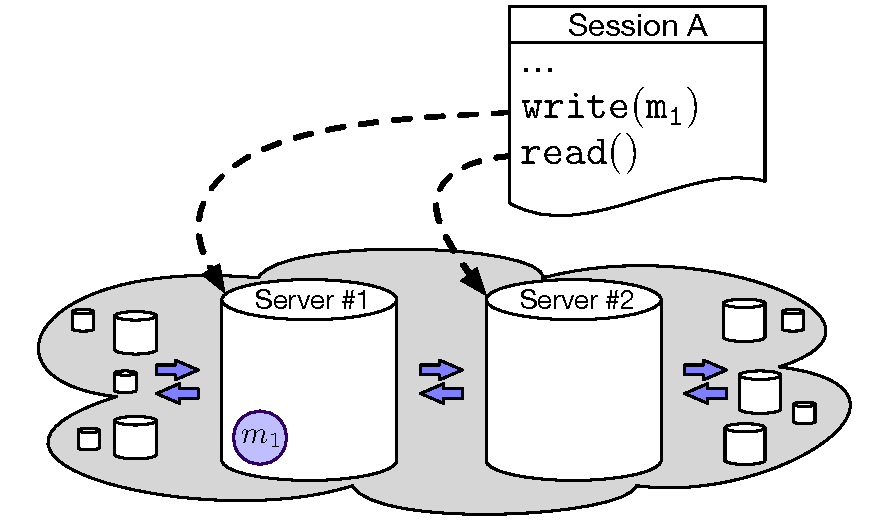
\includegraphics[scale=0.48]{../Figures/System_example.pdf}
\caption{A simple way of showing contracts}
\label{fig:ctrt}
\end{figure}


% Here, developers are forced to come up with their own implementation of
% RMW. They must modify client and server applications to generate, send
% and receive special tokens, to maintain the set of updates available at
% each server, and block user requests, if some necessary updates are
% still missing. Now, in order to have a correct application, the
% developer must prove certain non-trivial safety and liveness
% properties for this implementation. To make the matter worse, the
% proof will becmoe obsolete after each modification in the application or
% the consistency requirements. For example, after users reporting some unaccepatble
% behaviors, in order to disallow those executions, developers 
% implement and add another consistency guarantee to RMW; a task that
% would clearly make the original correctness proofs obsolete. 




% In this paper, we address these issues by introducing a compositional, principled approach to 
% derive enforcement mechanisms for various forms of weak consistency 
% guarantees. 
% We offer developers with a tool that generates a shim layer that works
% with an eventually consistent store and extends it to a key-value store
% with multiple environment, each of which shows a certain level of
% consistency, specified by the developers. 
% We also introduce a language for specifying application-level consistency 
% requirements as logical formulae that express legal execution states of the distributed store. 
% Our consistency enforcement methodology is independent of the underlying store 
% and only assumes the well-established guarantee of "eventual delivery". 
% Moreover, our enforcement tool is complete for the specification
% language, which itself is powerful enough to express all the known consistency 
% guarantees in the literature.

% We argue that all the consistency guarantees basically specify, \emph{when} an 
% application instance should block a user request and for arrival of 
% \emph{what} remote updates it should wait. For obvious reasons, any implementation of these 
% consistency guarantees must be \emph{correct} and \emph{optimal}. The former property states that 
% all possible behaviors of the implementation are allowed by the given specification and the later 
% ensures that application instances do not engage in 
% any unnecessary synchronization before responding to a user request (i.e. users are only blocked if 
% it is absolutely necessary).
% \\ Our technique is based on tracking relationships between update effects, and maintaining multiple 
% (logical) caches at the shim layer, each of which is enforced to satisfy a specific level of consistency, 
% derived from the given specifications. We believe that our approach is the first ever principled 
% reasoning and implementation framework for weak consistency enforcement techniques which 
% is also proven to be \emph{correct} and \emph{optimal}. 
% By separating all the consistency management procedures from the application level, we are taking 
% the non-trivial task of proving soundness criteria for ad-hoc consistency enforcement techniques 
% off of the developer's shoulders. 
% Contributions of the paper
A summary of our contributions is given below:
\begin{itemize}
\item Introducing a new specification language that covers all the known consistency guarantees in 
the context. Our language is arguably simpler than the previous proposals, and is based on observing 
similarities of different consistency requirements.

\item Proposing a principled consistency enforcement methodology that is 
complete for our specification language and allows deriving multi-purpose consistency enforcement 
tools.

\item Presenting proofs of correctness and optimality of our consistency enforcement technique
and introducing the first ever general reasoning framework for weak consistency guarantees. 

\item Introducing a tool called  \tool that realizes our consistency enforcement methods and 
extends an off-the-shelf eventually consistent data store (Cassandra) to a multi purpose key-value 
data store with the ability of guaranteeing any requested consistency level defined by the 
developers. 

\item Presenting the evaluation results showing the necessaity of
developing fine-grained weak consistency levels and the complexities
assosiated. Lastly, the utility of our tool is shown by comparing it to a hand-written
implementation of a weak consistency guarantee. 
\end{itemize}

Rest of the paper is organized as follows.  In section
Sec.~\ref{sec:motivation} we expand on the motivation of this work
with help of a detailed example. In Sec.~\ref{sec:contract-lang} we
introduce the abstract store model that forms the basis of our
specification language, along with the language itself. In
Sec.~\ref{sec:formalization}, we describe the semantics of our
consistency enforcement runtime, and formalize its correctness and
optimality guarantees. Sec.~\ref{sec:algorithm} elaborates on the
algorithmic aspects of our runtime key to its efficient realization.
Sec.~\ref{sec:evaluation} describes \tool, our implementation of the
specification language and enforcement runtime, and evaluates its
applicability and practical utility.  Related work and conclusions are
presented in Sec.~\ref{sec:related-work}.

%================================ SECTION TWO: System Model
\newpage
%==========================================================
%--- What programs are and how they are written in our tool
%==========================================================
\section{System Model}
\label{sec:sys_model}
In this section, we formally describe our system model, including the
notions of distributed applications and replicated data objects,
behavioral properties of eventually consistent data stores and
consistency guarantees.


A data store in our system model is a collection of \emph{replicas}
(\#1,\#2,...),
each of which maintains an instance of a set of  replicated \emph{data
object} ($x$,$y$,...).
The data objects,
which are defined by application developers, contain a \emph{state}
($v$,$v'$,...) and
are equipped with a set of \emph{operations} ($op$,$op'$,...), whose
type is either
read-only or effectful. 
The former type refers to the operations that just request reads from the
store, which are responded with an instance of the requested objects' state and the
latter refers to the operations that modify an objects' state by generating
an \emph{update effect} ($\eff$,$\eff'$,...).  Update effects or simply effects
are defined by
developers and are associated with an \emph{apply} function that enables
the asynchronous modification of the objects' state at different replicas.
The effect generated after an operation is submitted to a replica, is
simply written in the data-store, that guarantees
their eventual delivery to all the replicas. Each recipient replica then
uses the apply function to modify its local instance of the objects'
state  (Fig.\ref{fig:system_model}).

Observe that there is no direct synchronization between replicas when an
operation is being executed, which means there can be conflicting
updates on an object, that are generated at different replicas
concurrently. 
We do not bound the system to a particular
conflict resolution strategy but instead require developers to implement
their own desired approach within the apply function. This system model
admits all the inconsistencies associated with eventual consistency, and
as we will explain in section \ref{sec:motiv}, our tool equips users
with infrastructures to specify and prevent all those inconsistencies.

Clients interact
with the store by invoking operations on objects, where a \emph{session} is
the sequence of operations invoked by a particular client. Consequently,
operations
(and update effects) can be uniquely identified by
their invoking \emph{session id} and their \emph{sequence number} in
that particular session. The data store is typically accessed by a large
number of clients concurrently and as a result of the load balancing
regulations of the store, operations might be routed to different replicas,
even if they are from the same session (Figures \ref{fig:sys_model1} and
\ref{fig:sys_model3}).

We new define two relation over effects created in the store.
\emph{Session order} ($\xrightarrow{\soZ}$) is an irreflexive, transitive relation that relates
effects from the same session following the  integer \emph{smaller than} relation
over their sequence numbers.
Finally, \emph {visibility} is an
irreflexive and assymetric relation, which is written as ($\eff
\xrightarrow{\visZ} \eff'$) if at the generation time of $\eff'$ in a
replica, $\eff$ is
already arrived and applied at that replica (in Fig.\ref{fig:sys_model3} for example, for $\eff'$ (the effect of executing
op') we will have $\eff \xrightarrow{\visZ} \eff'$, since $\eff$ is
already present at the replica4, when op' is submitted).
\begin{figure}[t]
    \centering
    \begin{subfigure}[t]{0.31\textwidth}
    \centering
        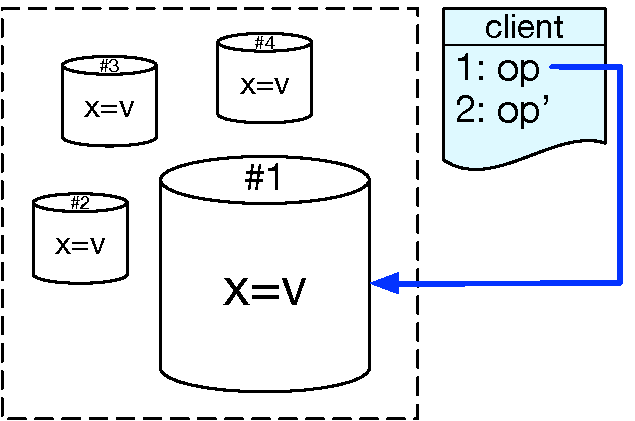
\includegraphics[scale=0.32]{Figures/system_model1.pdf}
        \caption{\scriptsize A client submits an operation op to the store, which
	is routed to the replica1.}
        \label{fig:sys_model1}
    \end{subfigure}
    \hfill
    \begin{subfigure}[t]{0.31\textwidth}
        \centering
	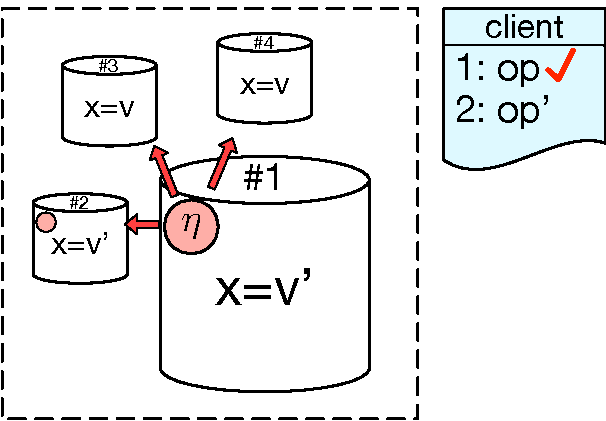
\includegraphics[scale=0.32]{Figures/system_model2.pdf}
        \caption{\scriptsize The state of the eplica1 is updated, an
	effect is created and is being propagated}
        \label{fig:sys_model2}
    \end{subfigure}
    \hfill
    \begin{subfigure}[t]{0.31\textwidth}
        \centering
	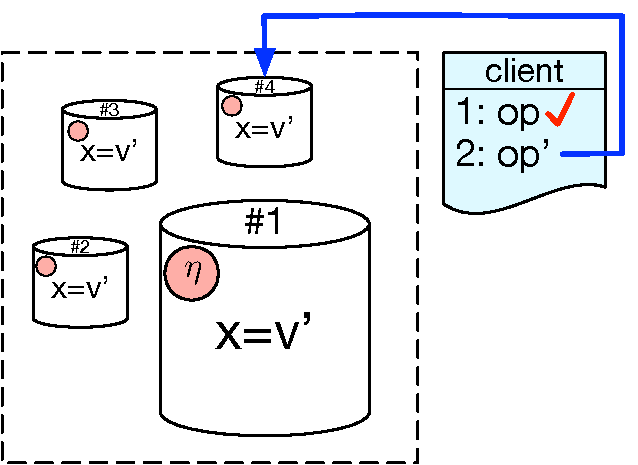
\includegraphics[scale=0.32]{Figures/system_model3.pdf}
        \caption{\scriptsize Second operation op' is submitted to the store, which
	is routed to another replica}
        \label{fig:sys_model3}
    \end{subfigure}
    \caption{system model of \tool}\label{fig:system_model}
\end{figure}




















%==========================================================
\newpage































































\begin{comment}

%
% Initial Paragraph explaining the running example
%

Let's consider the developement of a modern-day large scale \emph{Bulletin
Board} web application, that allows managers to initiate multiple boards for their
organization, where employees can either write something on the
board, or request to read all the messages on it.
In order to achieve high availablity, developers decide to implement the
application as distributed servers, working
with replicated data objects on top of an 
Eventually Consistent Data Store ({ECDS}). The data model here dictates
each row at the data base level, to include a board identifier
and a set of messages 
(Fig. \ref{fig:simple_bb}).
In this fashion, employees can start a session to send requests to geographically distributed
servers and make updates to the rows, and the underlying store,
would guarantee the eventual delivery of all updates at every server.
\begin{figure}[t]
    \begin{subfigure}[b]{0.48\textwidth}
        \centering
	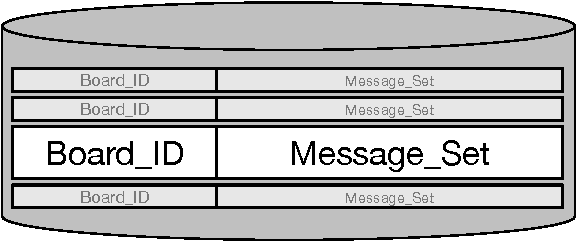
\includegraphics[scale = 0.5]{Figures/SimpleBulletinApp.pdf}
	\caption{Simple Data Model}
        \label{fig:simple_bb}
    \end{subfigure} 
    \begin{subfigure}[b]{0.48\textwidth}
        \centering
	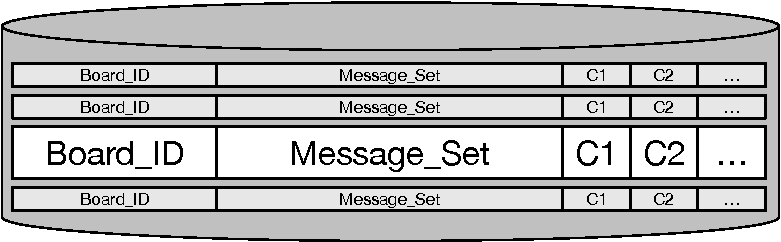
\includegraphics[scale=0.5]{Figures/ModifiedBulletinBoard.pdf}
	\caption{Modified Data Model}
	\label{fig:modified_bb}
    \end{subfigure}
    \\ \hrulefill \\
\caption{Low-Level Data Model of a Simple Bulletin Board Application
(Left) and the Modified Version Including Meta-data for Each Running
Session}
\label{fig:simple_modified_bb}
\end{figure}

%
%===========================================================================SUBSECTION
% Paragraph 2: Explaining the possible anomaly under EC
%
\subsection{Ad-hoc Anomaly Prevention Mechanisms}

Developers cannot solely rely on the eventual consistency guarantee that
is provided by the underlying data stores for application correctness. There are application integrity anomalies
that must be thought of at the developement stage and be handled. For
example, assume an employee signs into the system, writes some
messages on the board, and immediately refreshes her browser hoping to see
her messages on the board, which are however not there. This is obviously
not desirable and as mentioned in
the previous section,  can occure if
the write messages were sent to a server, and the subsequent read to
another, where her previous write updates are  not available yet. 
\begin{wrapfigure}{l}{0.3\textwidth}
	\centering
	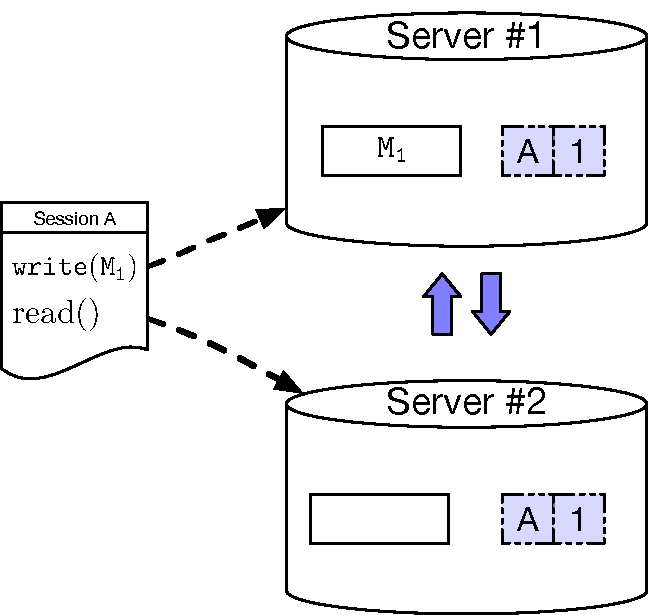
\includegraphics[scale = 0.4]{Figures/metadatapresent.pdf}
\vspace{1 mm} 
\hrule
\caption{Incorrect implementation of RMW. The meta data referring to the
first operation of session A can be present at server \#2, when the
actuall message is not}
\end{wrapfigure}

%
% Paragraph 3: Ad-hoc prevention methods
%

To prevent this anomaly, developers must provide RMW consistency
guarantee for their application, where user requests sent to a server are guaranteed to see
all the previous updates made by the same client and session. The
conventional technique for acheiving this,
is to tag each session and its contained requests, respectively with unique identifiers and
sequence numbers and to include this meta-data in the database, to
record what requests have been seen by the server at any time. 
Moreover, there must be some mechanisms to temporarily block user requests, when the database
does not include the updates from previous requests.
Since developers are not interested in synchronized and direct
communication between servers (which obviously contradics the idea of using
an ECDS), they have to record the meta data in the key value store and rely on
the provided delivery mechanisms. 
%
%Paragraph 4: The problem with simply adding the metadata on top of the
%implementation
%

However, the desired behavior cannot
be achieved by simply creating meta data "add-ons" to the current implementation.
The reason is that, in EC stores, no order of delivery is guaranteed,
and some servers might receive the meta-data regarding some updates that
are not present at the server yet. 
Developers need to make sure that the meta-data recording sequence
number of a request, becomes available at a server, at the same time
when the corresponding update arrives. This can only be done by
modifying the low-level initial data models, to also record the sequence
numbers seen from each client. 
%
% Paragraph 5: The difficulties of low-level modifications: complex
% and redundant
%

Now developers are inevitebaly required to modify the origianl low level
data model to also include the required meta data, so the changes in the
data and meta-data would arrive at servers atomically. Such changes on
the data model will require rewriting 90\% of application functions from the scratch
which is extremely inconvinience. 
Moreover, now developers must face non-trivial problems associated with
session management and dynamic data models. For example, when a new
client arrives at a server 
and initiates a session, the server is required to generate a unique ID
for that session, and then add a new column to the
underlying database table, to record the associated meta-data.
Unfortunately, table alteration in ECDSs is not an atomic task, and forces developers to implement
appropriate guards to make sure that the new column is available at all servers, before
allowing the client to move on with the rest of her requests.  
%
% Paragraph 6: The problem of new consistency requirements
%

To make the matter worse, new integrity anomalies are discovered very
frequently. Assume the bulltin board application with RMW has been
successfully designed and implemented, however, after the developement
phase users report a new type of anomaly, where messages seem to be
disappeared after refreshing the browser. This undesirable behavior is
allowed under EC and even RMW; since two read operations can go to
different servers, where the second one does not include all the
messages read from the first server. This requires another consistency
level, called Monotonic Reads, that guarantees subsequent reads will
include everything that has been read before in a session.
 
 
 






\end{comment}




%================================ SECTION THREE: Motivation
\newpage
\section{Motivation}
\label {sec:motiv}
In this section, we explain the developement process of a highly
available application in \tool. We discuss a possible  anomily under
eventual consistency and then explain the difficulties associated 
with the manual approaches for prevention techniques.
Lastly we will explain how by automating the process, \tool can liberate
the developers from all those problems.
Our ideas mentioned here, are completed in  section
\ref{sec:ctrt_language}, where we extend the tool with a language, to
specify \emph{any} kind of anomalies. 


%
%--- What is the application, what are the requirements 
%
\subsection{RDTs in Eventually Consistent Stores }
\begin{figure}[t]
        \centering
	\begin{subfigure}[b]{0.489\textwidth}
	\begin{lstlisting}
type Effect = String 
type State =  String 

read :: State -> (String,Maybe Effect)
read s = (s,Nothing)

write :: String -> ((),Maybe Effect)
write comment = ((),comment)

apply :: State -> Effect -> State 
apply s eff = in s ++ " - " ++ comment
	\end{lstlisting}
	\caption{A simple implementation}
	\label{subfig:comment_code}
	\end{subfigure}
	\hfill
	\begin{subfigure}[b]{0.475\textwidth}
	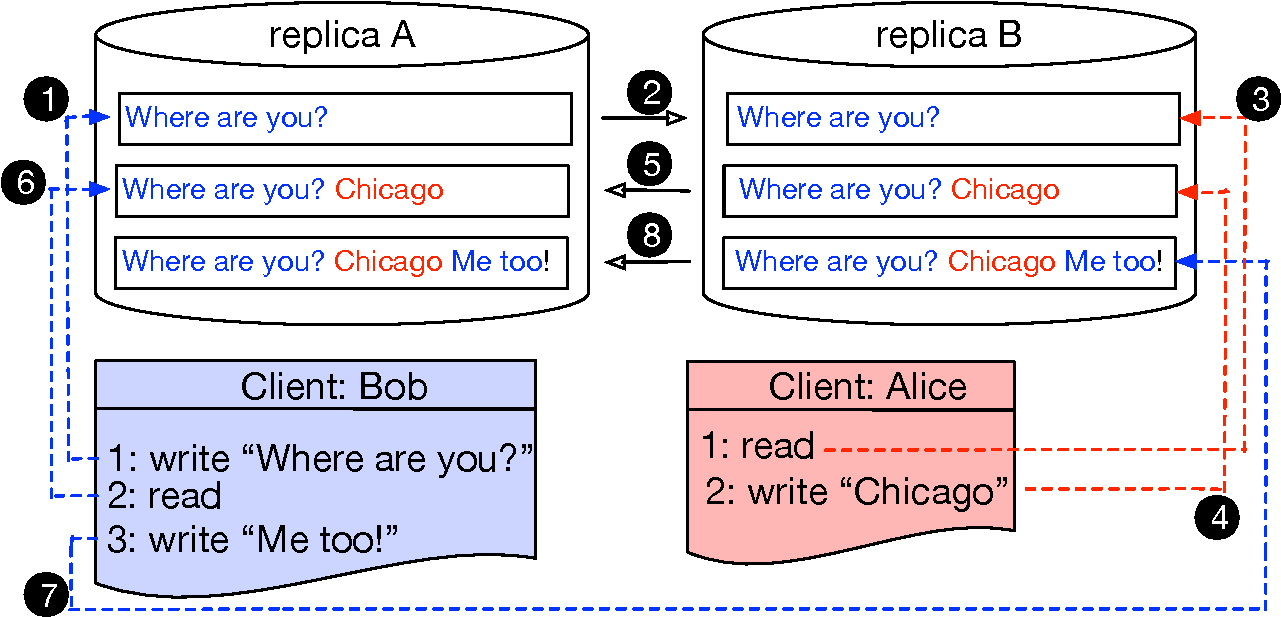
\includegraphics[scale=0.282]{Figures/comment_application.pdf}
	\caption{Example execution}
	\label{subfig:comment_example}
	\end{subfigure} 
\\ \hrulefill
\caption{A distributed application for comment section
management}
\label{fig:comment_app}
\end{figure}



Let's now consider a highly available comment
section management application, as part a photo sharing web site.
Figure \ref{subfig:comment_code} presnets implementation of such an application
in our system model. As explained in section \ref{sec:sys_model}, the
code is consisted of types \effectC{} and \stateC{}. Both types here are
defined as a strings, the former representing the text of a comment, and
the latter all the visible comments concatinated together.
Everytime a user calls the \writeC{} function to add a comment, an
\effectC{}
is generated and a \readC{} call simply
returns the \stateC{} of the object.

The \applyC{} function is given an effect, and is defined by the
developers to \emph{update} the objects' state.
Here the \applyC{} function simply pastes the 
included comment inside of  an effect, to the end of the current \stateC{}. As we mentioned earlier, we
completely separate the convergence semantics of the application  from the consistency
requirements. Since our focus is consistency here, we omit any conflict
resolution strategy in the code, however, developers (using roll-backs,
etc) can design the \applyC{} function to resolve conflicting
concurrent updates as they desire. 

Figure \ref{subfig:comment_example}, presents an example of how users
interact with the application. The example shows two clients, Bob and
Alice, that invoke operations on a comment section object. In the
setting Bob first writes a comment, which is routed to the replica A,
whose effect is then propagated and delivered to the replica B, where Alice's
first read operation is routed to next. Alice and Bob then keep talking
through more read and write events, whose order are marked in the
figure. 

Now let's assume Bob's read opration, instead of replica A, was routed
to another replica C, where the update from his first operation was not
present. This is \emph{lost-updates} anomaly, a very well-known
undesired behavior that is admitted in eventually consistent stores. 
Now developers are faced with the problem of preventing such an undesired
behavior, a task that as we will explain shortly, is difficult,
erorneous and heavily tangled with the application logic.
%
%--- What are the challenges implementing those reuquirements manually
%
\subsection{Ad-hoc Anomaly Prevention}
In this part, by referring to the modified code  presented in figure
\ref{fig:modified_code}, we will
explain a well-understood approach toward eliminating the lost\_update anomaly in
our comment manager application running on an EC store.

%tagging effects
First modification required in this technique is tagging effects with
unique identifiers, consisting their originating sessions' id, and their
sequence number in them. This is used by replicas to
record the set of effects, that are alerady present locally
($line:1,2,5$). By this simple adjustment, the undesired anomaly would
be completely avoided, if operations would never be routed to replicas,
that do not contain all the effects from prior operations on that
session (let's call these effects the dependencies of
the operation). 

%blocking
Since operations do not have any control on which replica they are
routed to, the above property can be achieved, if operations that are
routed to a replica that does not contain their dependencies, wait
before execution until such effects become available at that replica.
This technique that is called {\bf blocking}, guarantees that the state
witnessed by oerations, 
is updated by a set of effects that is a \emph{superset} of the desired
dependencies.

Moreover, another technique called {\bf filteration} is used to further realize
the above idea. It basically separates the set off effects that have
arrived to the replica (available effects), and the effects who have
arrived and also been applied to the state (filtered effects).
By this separation, replicas can only apply effects to their state, if all
effects in session order with them, have already been applied to the
state. 
This way, replicas can record only the highest sequence
numbers from each session that they have applied to the state (since it
is guaranteed that the smaller ones are also applied)($line:3,6$). 
Figure \ref{fig:modified_code}, represents the blocking technique in the modified \readC{}
operation, where the result is only returned if the required
dependencies have already been applied to the state. Furthermore, the
filteration technique is used bu tge modified \applyC{} funciton, only
updates the state, if the sequence number of the given effect is
larger than the highest previously applied effect to the state precisly
by 1.
\begin{figure}[t]
	\centering
	\begin{subfigure}[t]{0.5\textwidth}
	\begin{lstlisting}
data Sess = Bob | Alice
type ID = (Sess,Int) 
type Effect= (ID,String)
type State = (String,Int,Int)
	
read :: ID -> State -> String
read (sess,seq) (st,sq1,sq2) = 
	case sess (*@\textcolor{blue}{of}@*) 
		Bob ->   if (seq==sq1+1) (*@\textcolor{blue}{then}@*) st
		         else read (sess,seq)(st,sq1,sq2)
		Alice -> if (seq==sq2+1) (*@\textcolor{blue}{then}@*) st
		         else read (sess,seq)(st,sq1,sq2)
	\end{lstlisting}		  
	\end{subfigure}
	%
	\hfill
        %
	\begin{subfigure}[t]{0.42\textwidth}
	\begin{lstlisting}[firstnumber=13]
	apply :: State -> Effect -> State 
	apply (st,sq1,sq2) ((sess,seq),cm) = 
	  case sess (*@\textcolor{blue}{of}@*) 
	    Bob ->   if (sq1==seq-1)
	             (*@\textcolor{blue}{then}@*) (st++cm,sq1+1,sq2)
	             else (st,sq1,sq2)
	    Alice -> if (sq2==seq-1)
	             (*@\textcolor{blue}{then}@*) (st++cm,sq1,sq2+1)
	             else (st,sq1,sq2)
	\end{lstlisting}		  
        \end{subfigure}

	\hrulefill
	\caption{Guarded Application to Prevent Lost-updates Anomaly
	When Serving Bob and Alice}
	\label{fig:modified_code}
\end{figure}




The above approach although is shown to work correctly, but as our
example showed, requires fundamentall changes in the code where 90\% of
the application was rewritten. Additionally, the modifications are
heavily tangled with the application logic which is problem for
developement of and reasoning about large
productions.

However, the major drawback of this approach is the fact that requires
constant alterations in the state of the application when the sessions
come and go. The application is now required to make
sure that a new field is created locally \emph{and} globally when 
new sessions are connected. This can extremely degrade the performance
of the system since it requires direct synchronization between replicas.
We have shown in detail how this adversely effects the performance in section
\ref{sec:eval}, where  we explain our experience in implementing
such an ad-hoc approach.

To make the matter worse, in addition to the above difficulties,
new anomalies are constantly found in the system, which requires
developers to come-up with non-trivial solutions. For example, in the
above application, another type of anomaly can occur when a third user
Chris, uses the application and submits a read, which is routed to a
replica C, which only contains the write from Alice. Then Chris sees a
window containing "Chicago" message which does not make any sence.
{EXAMPLE SHOULD
BE EDITED *********}



%
%--- What is our alternative approach
%
\subsection{An Alternative}
use \tool!





















\newpage























%================================ SECTION FOUR: Specification Language
\section {Specification Language} 
\label{sec:ctrt_language}
\begin{figure}[t]
\begin{subfigure}{0.41\textwidth}
\centering
  \begin{fmathpar}
  \begin{array}{lclcl}
		\rel & \in & \texttt{rel.seed} & \coloneqq & \visZ \ALT
		\soZ \ALT \rel \cup \rel \\
               \Rel & \in & \texttt{relation} & \coloneqq &  \rel
	       \ALT \Rel;\rel  \ALT \nullR  \\
	     \pi & \in & \texttt{prop} & \coloneqq & \forall a.
      ~a \xrightarrow{R} \hat{\eff} ~\Rightarrow~ a \xrightarrow{\visZ}
      \hat{\eff}\\
		\psi & \in & \texttt{spec} & \coloneqq & \pi \ALT \pi \conj \pi
  \end{array}
  \end{fmathpar}
\subcaption{ syntax of contracts}
\label{fig:ctrt_syntax}
\end{subfigure}
\hfill \vline \hfill
\begin{subfigure}{0.49\textwidth}
\centering
\begin{scriptsize}
\begin{tabular}{|l | c |} 
\hline
 { \texttt Guarantee} & {\texttt Contract} \\ [0.5ex] 
\hline 
\textsc{Read My Writes} & $\forall a. a ~  ~\xrightarrow{\soZ}  ~ ~
\hat{\eta} \Rightarrow a \xrightarrow{\visZ} \hat{\eta} $ \\ 
\textsc{Monotonic Writes} & $\forall a. a \xrightarrow{\soZ;\visZ}
\hat{\eta} \Rightarrow a \xrightarrow{\visZ} \hat{\eta} $ \\ 
\textsc{Monotonic Reads} & $\forall a. a \xrightarrow{\visZ;\soZ}
\hat{\eta} \Rightarrow a \xrightarrow{\visZ} \hat{\eta} $ \\ 
\textsc{Transitive Visibility} & $\forall a. a \xrightarrow{\visZ;\visZ}
\hat{\eta} \Rightarrow a \xrightarrow{\visZ} \hat{\eta} $ \\ 

\hline
\end{tabular}
\end{scriptsize}
\subcaption{examples 
%({\bf R}ead {\bf M}y {\bf W}rites, {\bf M}onotonic
%{\bf W}rites and
%{\bf M}onotonic {\bf R}eads)
}
\label{fig:ctrt_example}
\end{subfigure}
\caption{\tool Specification Language}
\end{figure}

The formal syntax of our specification (or contract) language, presented in
Fig.\ref{fig:ctrt_syntax}, allows definitiosn of
\propS{}, a first-order formula
that establishes dependency relations between effects,
necessary to determine the effects an operation may witness, under
a given consistency level.
The language is seeded with $\soZ$ and $\visZ$, respectively representing session
order and visibility relations over effects, 
and defines dependency \relationS{} as a sequence\footnote{\tool also allows
using closures of seeds, which is omitted here for
simplicity.} of seeds,  
where 
({\footnotesize $a \xrightarrow{\rel_1;...;\rel_k} b$})
is interpreted as 
{\footnotesize$\exists c. (a
\xrightarrow{\rel_1;...;\rel_{k-1}} c
\wedge c \xrightarrow {\rel_k} b)$}.
$\nullR{}$ is the empty relation.
Additionally, the language allows conjunctions of propositions, \specS{},
used to define a safe environment
free from \emph{multiple} inconsistencies. 
Our language is crafted to capture all fine-grained weak consistency
levels, including well-known ones such as those explicated by Terry et al. \cite{terry}
(see e.g., Fig.\ref{fig:ctrt_example}).

%
% UB and LB contracts
We provide two important classes of 
contracts, and explain how they can be
satisfied with different enforcement techniques.
\begin{description}
\item {\textsf LB}: A \emph{lower bound} (\LB{}) contract is one in
  which all defined dependency relations end with an \soZ, i.e. are of
  the following form: ({\footnotesize $\forall a. a
    \xrightarrow{r_1;r_2;...;\soZ} \hat{\eff} \Rightarrow a
    \xrightarrow{\visZ} \hat{\eff}$}). It specifies the smallest set
  of effects that any operation should witness to maintain
  consistency, e.g.  \rmwCTRT{} and \mrCTRT{} in
  Fig.\ref{fig:ctrt_example}.

\item {\textsf UB}: Similarly, we define \emph{upper bound} (\UB{})
  contracts as those whose dependency relations end with a $\visZ$.
  These contracts define constraints on the set of effects made
  visible to each operation; if an effect is in the set, certain
  dependencies of that effect must also be included, e.g.  \visCTRT{}
  and \mwCTRT{} in Fig.\ref{fig:ctrt_example}.
\end{description}
Our consistency enforcement approach is based on blocking operations
with \LB{} contracts to make sure that they witness \emph{all effects
  that they are supposed to}, and filtering for \UB{} contracts to
make sure that they do not witness \emph{effects that they are not
  supposed to}.  


%================================ SECTION FIVE: Semantics
%========================================================================================================================
%========================================================================================================================
%========================================================================================================================
\section{Semantics}
\label{sec:semantics}
In this section, we present the consistency enforcement mechanism of
\tool, abstracted as a formal operational semantics. Our approach is
complete for the specification language defined in
Sec.\ref{sec:ctrt_language}.  However for better comprehensibility, we
present the semantics and the theorems paramterized over a contract
consisting of a single proposition.  Therefore, in the rest of this
section, we will assume a given contracat $\psi$ of the following
form:
\begin{fmathpar}\footnotesize
\begin{array}{lll}
\psi = \forall a. a \xrightarrow{\rel_1;\rel_2;...;\rel_k} \hat{\eta} \Rightarrow a 
\xrightarrow{\visZ} \hat{\eta}
&\qquad 
\quad & \rel_i \in \{\visZ;\soZ\}
\end{array}
\end{fmathpar}
%
%

The operational semantics defines a small-step relation over \emph{execution
states}, which are tuples of the form {\footnotesize $\E=(\EffSoup,\visZ
,\soZ)$}.
The \emph{effect soup} $\EffSoup$ stands for the set of all
effects produced in the system, and \emph{primitive relations}
{$\visZ,
\soZ \subseteq \EffSoup \times \EffSoup$}, respectively represent the
visibility and session order 
among such effects. Figs.~\ref{subfig:execution_graph} and
\ref{subfig:execution_example} present a simple
execution state consisting of 9 effects with associated
primitive relations\footnote{We omit drawing transitive $\soZ$
edges (e.g. between
$\eff_8$ and $\eff_1$) for better readability.}.
\begin{figure}[h]
	
	\begin{subfigure}[b]{0.28 \textwidth}
	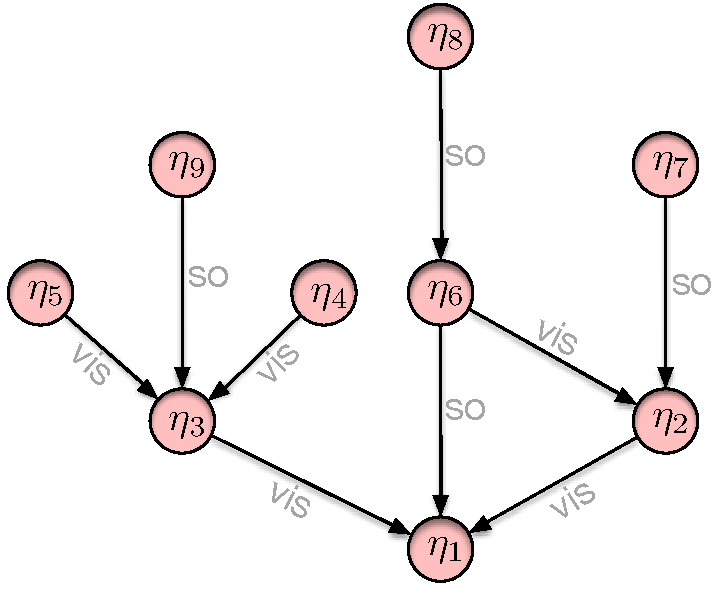
\includegraphics[scale=0.38]{Figures/execution.pdf}
	\subcaption{An execution state \E}
	\label{subfig:execution_graph}
	\end{subfigure}
	%
	\quad \vrule \quad
	%
	\begin{subfigure}[b]{0.31 \textwidth}
	\begin{smathpar}
	\begin{array}{lcl}
	\E.\EffSoup & = & 
	\{\eta_1,\eta_2,\eta_3,\eta_4,\eta_5,\eta_6,\eta_7,\\ & & \;\eta_8,\eta_9\}\\
	\E.\visZ & = & 
	\{(\eta_5,\eta_3),(\eta_4,\eta_3),(\eta_3,\eta_1),\\ &
	&\;(\eta_2,\eta_1),(\eta_6,\eta_2)\} \\ 
	\E.\soZ & = & \{(\eta_9,\eta_3),(\eta_8,\eta_6),(\eta_6,\eta_1),\\ 
	& & \;(\eta_8,\eta_1),(\eta_7,\eta_2) \} \\ 
	\end{array}
	\end{smathpar}\\
	\subcaption{Effect soup and primitive relations}
	\label{subfig:execution_example}
	\end{subfigure}
	%
	\quad \vrule \quad
	%
	\begin{subfigure}[b]{0.3 \textwidth}
	\begin{smathpar}
	\begin{array}{lll}
	\visZ^{-1}  (\eta_1) & = & \{\eta_2,\eta_3\} \\ 
	\soZ^{-1}  (\eta_1) & = & \{\eta_6, \eta_8\} \\
	(\soZ\cup\visZ)^{-1} (\eta_1) & = &
	\{\eta_2,\eta_3,\eta_6,\eta_8\} \\ 
	(\visZ^*)^{-1} (\eta_1) & = &
	\{\eta_2,\eta_3,\eta_4,\eta_5,\eta_6\} \\ 
	(\soZ;\visZ)^{-1}(\eta_1) & = & \{\eta_7,\eta_9\}
	\\ \\
	\end{array}
	\end{smathpar} \\
	\subcaption{Relation inverse examples}
	\label{subfig:inverse_example}
	\end{subfigure}
	\caption{A simple execution state }
\label{fig:execution_state}
\end{figure}

We denote the subset of $\EffSoup$ consisting of effects that
satisfy a certain condition as $\EffSoup_{(\mathtt{condition})}$.

% models
Note that \tool's contracts are in fact constraints over execution states,
where the domain of quantification is fixed to the effect soup
$\EffSoup$, and
interpretation for $\soZ$ and $\visZ$ relations (which occur free in the
contract formulae) are also provided. Thus, execution states are
potential models for any first-order formula expressible in the
specification language. If an execution state $\E$ is a valid model
for a contract $\psi$, we say that $\E$ satisfies $\psi$ ($\E
\models \psi$). 

%reduction relation
The reduction relation in our semantics is of the form
{\footnotesize $
(\E,\op_{<s,i>}) \;\xrightarrow{V}\; (\E', \eff),
$}
which can be interpreted as a transformation of the initial execution state
$\E$, caused by a replica with a local 
set of effects $V$, when it executes
$\op$, the $i^{th}$ operation from the session $s$. 
During this reduction step, a new effect $\eff$ is produced and added to
the system, resulting in a new execution state $\E'$ composed of an updated effect
soup and new primitive relations.





%=============================================================================================================
%=============================================================================================================
%--------- Definitions to be used in the semantics
%=============================================================================================================
\subsection{Preliminaries}
\label{subsec:prelim}
Before presenting the operational semantics, we first introduce
supporting definitions and notations.
We start by defining the interpretation of an \emph{inversed} 
dependency relation 
{\footnotesize $\Rel^{-1}$} under an execution state $\E$, 
which is utilized in the basis of our consistency enforcement mechanism.
We previously mentioned our interpretation for $\soZ$ and $\visZ$
between
effects under  $\E$; this can now be straightforwardly extended to their inverse as
follows\footnote{Note that when the input of an inversed relation is a singleton
$\{\eta\}$, we drop the brackets and simply write it as
$\rel^{-1}(\eta)$}:
\begin{equation}
\label{eq:r_inv}
\scriptsize
\rel^{-1}(S) = 
\begin{array}{lcl}
\bigcup\limits_{b\in S}\{a|(a,b) \in \E.\rel \} & \qquad & \rel\in\{\soZ,\visZ\}
\end{array}
\end{equation}
Additionally, based on our interpretation of the sequences of seed
relations given in Sec.\ref{sec:ctrt_language}, we can
extend the above definition:
\begin{equation}
\label{eq:seq_inv}
\scriptsize
\begin{array}{lllll}
b \in  (\Rel';\rel)^{-1}(a) & \iff & \exists c. c \in \rel^{-1}(a)
& \wedge & b \in (\Rel')^{-1}(c) 
\end{array}
\end{equation}
It might seem that we are ready to define any $\Rel^{-1}$ 
based on  the two definitions above; 
however, note that definition (\ref{eq:seq_inv}) fails to capture
the reality of our system model, where all computations are
performed by replicas independently; at any given moment, a replica might have access to only a
\emph{subset of all produced effects} in the system.
For example, consider  {\footnotesize$(\soZ;\visZ)^{-1}(\eta_1)$} under the
execution state presented in Fig.\ref{fig:execution_state}. 
In order to compute this set, based on (\ref{eq:seq_inv}) we have: 
\begin{smathpar}
\scriptsize
\begin{array}{lllll}
b \in  (\soZ;\visZ)^{-1}(\eta_1) & \iff & \exists c. c \in
\visZ^{-1}(\eta_1)
& \wedge & b \in (\soZ)^{-1}(c)
\end{array}
\end{smathpar}
%%%SJ: This is confusing.
Now, since there exists \emph{mid-level} effects $c=\eta_2$ and 
$c=\eta_3$,  that satisfy the above definition respectively 
for $\eta_7$ and $\eta_9$, we can conclude: {\footnotesize$(\soZ;\visZ)^{-1}(\eta_1) =
\{\eta_7,\eta_9\}$}.
Consider a replica that contains {\footnotesize$\{\eta_1, \eta_6, \eta_7,
\eta_9\}$} at the moment, and wants to check if the dependencies of $\eta_1$ are locally present 
or not. Even though based on the above definition, the
answer is affirmative (since the replica does contain $\{\eta_7,\eta_9\}$), 
the replica has no way to verify it, since the mid-level
effects $\eta_2$ and $\eta_3$ are not present at the replica yet. 

To capture the above property, we redefine the 
inverse of $\Rel$, \emph{according to a set of available effects $V$}, 
that considers whether all required mid-level effects are present in $V$.
The following definition is based on (\ref{eq:r_inv}) and a more
strict version of (\ref{eq:seq_inv}):
\begin{equation}
\label{eq:R_inv}
\scriptsize
b \in \Rel^{-1}_V(a) \iff
\begin{cases}
\begin{array} {lllll} 
\bot & \;\myif\; & \Rel = \nullR& & \\
b \in \rel^{-1}(a) & \;\myif\; & \Rel=\rel & & \\
\exists c. c \in
\rel^{-1}(a) \wedge b \in (\Rel')_V^{-1}(c) \wedge
\rel^{-1}(a) \subseteq V   & \;\myif\; & \Rel=\Rel';\rel & & \;
\end{array}
\end{cases}
\end{equation}
For example, in Fig.\ref{fig:execution_state}, 
{\footnotesize  ($\eta_9 \in
(\soZ;\visZ)_{\{\eta_1,\eta_3\}}^{-1}(\eta_1)$)}
holds, but {\footnotesize($\eta_9 \not\in (\soZ;\visZ)_{\{\eta_1\}}^{-1}(\eta_1)$)}. 

We define a set $V$ to be \emph{self-contained} for
a given effect $\eta$,
written as {\footnotesize $\SC
R \eta V$}, if $V$ contains all the required mid-level effects to compute
$R$ inverse of $\eta$ in totality, i.e.
\begin{equation}
\scriptsize 
\SC R \eta {V} \iff R^{-1}_V(\eta) = R^{-1}_{E.A}(\eta)
\end{equation}
For example in Fig.\ref{fig:execution_state}, {\footnotesize $\SC R
{\eta_1} V$} holds for an arbitrary  $R$ and for any $V$ that is a superset of
{\footnotesize $\{\eta_1,\eta_2,\eta_3,\eta_4,\eta_5\}$}.

We define {\footnotesize \trunc{}} as a function that
given  $R \in$ \relationS{}, 
returns a new relation by removing the last element from the sequence
in R:
\begin{equation}
\scriptsize
\trunc{R} = 
\begin{cases}
\begin{array}{lcl}
\nullR & \quad \myif \quad & R = \rel \quad \mathtt{or} \quad R = \nullR \\
R' & \quad \myif \quad & R = R';\rel 
\end{array}
\end{cases}
\end{equation}

Finally, we define \emph{closed subsets} of a given set $V$, 
as the subsets that are closed under {\footnotesize$(\trunc{R}^{-1}_V)$}, that
also contain all the required mid-level effects to compute
{\footnotesize $\trunc{R}^{-1}$}.
Moreover, we define the largest element among such
subsets, as the \emph{maximally closed subset} of V as follows\footnote{We slightly abuse the previously defined notation
in (\ref{eq:R_inv})
and use a \emph{set} of effects as the input of
$R^{-1}$, which is defined as:
$x \in R^{-1}_V(S) \iff \exists (y\in S). x \in R^{-1}_V(y)$.}:
%
\begin{fmathpar}
\begin{array}{rlllll}
\mathtt{closed \; subsets:} &  V' \in \left \lfloor  V \right \rfloor & \iff & V' \subseteq V & \wedge &
(\trunc R)_V^{-1}(V') \subseteq V' ~\wedge ~ \SC {\trunc{R}} \eta {V'}    \\
\mathtt{maximally \; closed \; subset:} & V' = \left \lfloor  V \right
\rfloor_{\mathtt{max}} & \iff & V' \in \left \lfloor  V \right \rfloor &
\wedge & \not\exists V'' \in \left \lfloor  V \right \rfloor. |V''|>|V'|
\end{array}
\end{fmathpar}






%=============================================================================================================
%--------- The operational semantics
%=============================================================================================================
\subsection{Core Operational Semantics}

\begin{figure}[t]
\raggedright
\textbf{Auxiliary Definitions}\\ \vspace{-2mm}
%
\begin{minipage}{0.5\textwidth}
\begin{fmathpar}
\begin{array}{lclcl}
  \multicolumn{5}{c}{
    {op} \in \mathtt{Operation\; Name} \spc \spc
    {v} \in \mathtt{Return\; Value} \spc \spc
    {s} \in \mathtt{Session\; Id} \spc\spc
  } 
  \\ 
  \eff & \in & \mathtt{Effect} & \coloneqq &  (s,op,v)\\
  F_{op} & \in & \mathtt{Op.\,Def.} & \coloneqq & \set{\eff} \mapsto v\\
  \EffSoup & \in & \mathtt{Eff\,Soup}	  & \coloneqq & \set{\eff} \\
  \visZ,\soZ &	\in & \mathtt{Relations} & \coloneqq & \set{(\eff,\eff)} \\
  {\E} 	& \in & \mathtt{Exec\;State}  & \coloneqq & \Exec \\
\end{array}
\end{fmathpar}
\end{minipage}
%

\vspace {3mm}

\textbf{Auxiliary Reduction} \; \\
\fcolorbox{black}{pgrey}{\scriptsize \(\auxred{S} {(\E,op_{<s,i>})} {} {(\E',\eff)}\)}\\
\begin{minipage}{0.9\textwidth}
\vspace{2mm}
\rulelabel{Oper}
\vspace{-2mm}
\begin{fmathpar}
\stretcharraybig
\begin{array}{l}
\RuleTwo
{
%\Theta(\rho \mapsto (v,cache)) \qquad
S \subseteq \EffSoup \qquad F_{op}(S) = v \qquad
\eta \not\in S \qquad
\eff = (s,op,v) \qquad  \\
%\id(\eta) = i \qquad
%\{\eff'\} = \EffSoup_{({\sf SessID}=s,\,{\sf SeqNo}=i-1)}\\
\EffSoup' = \EffSoup \cup \{\eff\}  \qquad
\visZ' = \visZ \cup S \times\{\eff\}\qquad
\soZ' = \soZ \cup \{(\eta',\eta) \,|\, \eta'\in \EffSoup_{({\sf
SessID}=s)}      \}\qquad
%\soZ' = (\soZ^{-1}(\eff') \cup \eff') \times\{\eff\} \cup \soZ
}
{
  \auxred {S} {((\EffSoup,\visZ,\soZ), op_{<s,i>}))}
  {} {((\EffSoup',\visZ',\soZ'),\eta)}
}
\end{array}
\end{fmathpar}
\end{minipage}
\vspace{4mm}\\
\textbf{Operational Semantics} \; \\
  \fcolorbox{black}{pgrey}{\scriptsize \((\E,op_{<s,i>}) \;\xrightarrow{V}\; (\E',\eff)\)}\\
\vspace{2mm}
\begin{minipage}{0.45\textwidth}
\rulelabel{UB Exec}
\vspace{-2mm}
\begin{fmathpar}
\stretcharraybig
\begin{array}{l}
\RuleTwo
{
  \visZ \subseteq r_k \spc
  V \subseteq E.A \spc  
  V'= \left \lfloor V \right \rfloor_V \spc
  \\ %   R^{-1}_{V}(\eta) \subseteq V' \\
  \auxred {V'} {(E, op_{<s,i>}))}
    {} {(E',\eta)} 
}
{
  (\E,op_{<s,i>}) \;\xrightarrow{V}\; (\E', \eff)
}
\end{array}
\end{fmathpar}
\end{minipage}
\hfill
\begin{minipage}{0.45\textwidth}
\rulelabel{LB Exec}
\vspace{-2mm}
\begin{fmathpar}
\stretcharraybig
\begin{array}{l}
\RuleTwo
{
     \visZ \not\subseteq r_k \spc
     V \subseteq E.A \spc  
     R^{-1}_{V}(\eta) \subseteq V \\
  \auxred {V} {(E, op_{<s,i>}))}
    {} {(E',\eta)} 
}
{
  (\E,op_{<s,i>}) \;\xrightarrow{V}\; (\E', \eff)
}
\end{array}
\end{fmathpar}
\end{minipage}
\\
\vspace{5mm}
\hrulefill\\
\caption{Core Operational semantics of a replicated data store.}
\label{fig:semantics}
\end{figure}

 %--- The Figure Containing the Rules
%--- Section intro
Our operational semantics is defined as a set of reduction rules
representing our consistency enforcement approach (see
Fig.\ref{fig:semantics}). The small-step reduction relation
($\rightarrow$) is parametrized over a set $V$, which stands for the
locally available set of effects at the replica taking the reduction
step.  Trivially, $V$ must be a subset of all effects in the system at
the initial execution state, however, there is no other restrictions
on $V$, since we only assume eventual consistency in the underlying
store.

%--- The Aux [OPER] rule
The rule
\rulelabel{oper} defines the abstract procedure of generating a new effect $\eff$, by witnessing a set
of effects $S$, using a user-defined function $F_{op}$. 
We formally define an effect as a tuple $\eff=(s,op,v)$, representing the
session $s$, operation name \emph{op} 
whose execution created $\eff$, and the value $v$
that the replica returns, responding to that operation.
%
Moreover, the rule explains how the execution state changes after a new
effect is produced. Specifically, in the new execution state, 
the effect soup
$\EffSoup'$ contains the newly created effect $\eff$,
the relation $\visZ'$
captures the fact that all effects in the set $S$ were made
visible to $\eta$, and $\soZ'$ states that all effects from the same
session as the current operation that are
already presenet in the system, should be in session
order with $\eff$ in the final execution state.

%--- rule for (->) relation
%UB
Rule\rulelabel{ub exec}, defines the execution of an operation in a
replica under a \UB{} contract.  The rule requires operations to only
witness $V'$, the maximally closed subset of $V$.  Thus,, the rule
governs how replicas create safe environments for operations, by
filtering out undesirable or uwanted effects.

%LB
Rule \rulelabel{lb exec} defines the step taken by a replica when an
operation is executed under an \LB{} contract. The precondition
$R_V^{-1}(\eff)\subseteq V$ in the rule ensures that the reduction
happens only if the effects necessary to avoid the specified anomaly
are present in $V$, assuming that $V$ contains all the mid-level
effects to determine dependencies of the newly created effect $\eta$
(i.e.  is a self contained set). Thus, the rule governs replicas to
block execution of an operation under an \LB{} contract, if the
replica is unable to verify the presence of all necessary dependent
effects.


%=============================================================================================================
%--------- Theorem on correctness of enforcement
%=============================================================================================================
\subsection{Soundness and Optimality}
\label{subsec:sound}
%
%Subsection on the correctness of contract 
%
In order to prove a meta-theoretic correctness property for our
semantics, we first define a $\psi$-consistent set of effects $S$ given
a execution state $\E$ as follows:

\begin{equation}
\scriptsize
S \mathtt{\;is\;} \psi \mathtt{-consistent} \iff \forall (\eff \in S).
\forall(a\in \E.\EffSoup). \trunc{R}(a,\eta)
\Rightarrow a \in S
\end{equation}
%Where the definition of $R$ is based on the definition of $R^{-1}$ from
%subsection 
%\ref{subsec:prelim}:
%\begin{equation}
%\scriptsize
%R(a,b) \iff a \in R_{E.A}^{-1}(b)  
%\end{equation}
\begin{theorem}
\label{theorem:one}
For all reduction steps 
$
\scriptsize
\; (\E,op_{<s,i>}) 
    \xrightarrow{V}
  (\E',\eff)  
$,
\begin{fmathpar}
\begin{array}{ll}
(i) & \mathtt{if\;} V \mathtt{\;is\;} \psi \mathtt{-consistent\;} \mathtt{under\;} \E,
\mathtt{\;then\;}  V \cup \{\eta\} \mathtt{\;is\;} \psi\mathtt{-consistent \; under\;} E'  \\
(ii) & E' \models \psi[\eta/\hat{\eta}]
\end{array}
\end{fmathpar}



\end{theorem}
\begin{proof}
Appendix \ref{app:proof1}
\end{proof}







%=============================================================================================================
%--------- Theorem on maxVis and minWait
%=============================================================================================================
%
%Subsection of the maximality of the set made visible and liveness
%properties 
%
\begin{theorem}
\label{theorem:two}
For all reduction steps
{\footnotesize $
(\E,op_{<s,i>}) 
    \xrightarrow{V}
  (\E',\eff) 
$},
the set of effects made visible to $\eta$ is maximal. i.e. for all
 {\footnotesize $a \in V$}, if 
 {\footnotesize $ \SC {\trunc{R}} a V$}, then 
\begin{fmathpar}
(a,\eta) \not\in \E'.\visZ \Rightarrow 
(\E'.A,\E'.\visZ \cup \{a,\eta\}, \E'.so) \not\models \psi[\eta/\hat{\eta}]
\end{fmathpar}
\end{theorem}


%
% THE MINIIMAL WAIT THEOREM
%

\begin{theorem}
\label{theorem:three}
For all execution states $E$, if there
exists ($S\subseteq E.A$) such that: 
\begin{smathpar}
\auxred{S} {(\E,op_{<s,i>})} {} {(\E',\eff)} \spc \wedge \spc (\mathtt{S \cup \{\eta\} \; is 
\;} \psi \mathtt{-consistent \; under \;} E' )  
\end{smathpar}
then there exist  $E''$, $\eff'$ and $V\subseteq E.A$ such that:
$((\E,op_{<s,i>})\;\xrightarrow{V}\;(\E'',\eff'))$
\end{theorem}
\begin{proof}
The proof is given by choosing set $V$ to be equal to $S$, and then
considering two cases, where either $S$ or $\left \lfloor S \right
\rfloor_S$ are made visible to operations, if the contract is respectively
waiting and non-waiting. In both cases, all premises of taking an step
are satisfied.
A detailed proof can be found in appendix
\ref{app:proof3}.
\\
\end{proof}


























% GENERALIZATION OF THE SEMANTICS WHICH I DONT THINK SHOULD BE INCLUDED
% BECAUSE OF LACK OF SPACE
%=============================================================================================================
%=============================================================================================================
\begin{comment}
%=============================================================================================================
%--------- How it can be generalized for all contracts
%=============================================================================================================
\subsection{Generalization}
\label{subsec:generalization}
We finish this section by extendeding our ideas in two dimentions. 
We will first explain how to handle an arbitrary
contract $\psi$ of the following form:  
\begin{fmathpar}
\psi = \pi_1 \wedge \pi_2 \wedge ... \wedge \pi_m \qquad \qquad 
\pi_i = \forall (a,b). a \xrightarrow{R_i} b \Rightarrow a
\xrightarrow{\visZ} b
\end{fmathpar}
Later, we will
explain how to maintain multiple levels of consistency simultaneously,
each of which is defined for a different operation name. We will assume an arbitrary contract
$\psi_{\op}$ for every user-defined operation $\op$, and explain how to
modify our system model to preserve them all.

To begin with, as we mentioned earlier, all propositions in our specification language,
either put a maximal or a minimal bound on the subset of local effects 
to be made visibe to each opreation. 
This simply means that when the system is given a conjunction
of propositions, it should define the such subsets in a way, so it would not violate
\emph{any} of them. 
Therefore, by a few modifications we can extend the system to support
all contracts. Firstly, the single premise $R_V^{-1}(\eta) \subseteq V$
in the reduction rule should be replaced with the following
conjunction: 
\begin{fmathpar}
\bigwedge_{1 \leq i \leq m} (R_i)_V^{-1}\subseteq V
\end{fmathpar}
Secondly, the definition of the maximal closed subset of local effects
must also be modified to a subset that is closed under \emph{all} given
relations:
%---------------------------------------------------------------------
% I am not sure if we should include the formal definition here. It is
% unnecessarily complex
\begin{fmathpar}
\left \lfloor S \right \rfloor_V = S' \spc \iff \spc S'
\subseteq S \; \wedge \;
\bigwedge(R_i)_V^{-1}(S') \subseteq S' \; \wedge \; 
\not\exists
S''.(\bigwedge ((R_i)_V^{-1}(S''))\subseteq S''\wedge |S''|>|S'|)
\end{fmathpar}
%---------------------------------------------------------------------

Moreover, for modifying the system to handle multiple contracts
simultaneously, we can
extend the local effect set $V$, to a sequence
of sets $V_{\op_i}$, each maintaning  the consistency level for an
operation type $\op_i$. Now we define the modified form of execution steps as
follow:
\begin{fmathpar}
(\E,\op_{<s,i>}) 
    \;\xrightarrow{V_{\op}}\;
  (\E',\eff) 
\end{fmathpar}
The local effect set $V$ must also be replaced with $V_{\op_i}$ in the 
premises of the reduction rules, so each operation of type $\op_i$ would
only witness the associated subset for its own consistency requirements.
This abstractly represents our implementation, in the sense that all operations
work only on a specific subset of available effects at any replica. The subset, is
maintained according to the contract assosiated with each operation, and
is guaranteed to preserve the consistency requirements following the
theorems of sections \ref{subsec:sound} and \ref{subsec:opt}. 
\end{comment}


%================================ SECTION SIX: Algorithm
\section{Implementation}
\label{sec:alg}
We implemented our tool as an extension to a GHC Haskell add-on, called
Quelea 
\cite{quelea},
previously developed by Sivaramakrishnan and two of the authors of this paper.
Quelea maintains a causally consistent cache on top of Cassandra, and \emph{all} operations whose contract is satisfied under causal
consistency, are performed witnessing that cache (even if they require considerably
weaker guarantees than causal).

In \tool, we maintain a generic cache equipped with a tagging mechanism,
where each operation is associated with a tag, and is allowed to witnesses only the subset of effects in the
cache, holding that tag (i.e. effects that are in the \emph{logical
cache} associated with that operation). We implemented a dependency finder mechanism in
\tool, that is used to verify the presence of arbitrarily defined dependencies of an
effect in each logical cache. Consequently, \tool's filtration and blocking
mechanisms are added to the runtime system, which rely on this dependency finder to keep each logical cache
consistent according to its associated contract. Specifically, 
considering a dependency relation $R$ and a replica containing a localset $V$
of effects, an effect $\eta$ is allowed to enter a logical cache, only if
$\trunc{R}_V^{-1}(\eta)$ is already in that cache. 


%the memoization technique
Considering the arbitrary length of the dependency relations expressible
in our contract language, and the fact that verifying the presence of
dependancies for an effect might fail for an unbounded number of trials
until all the dependencies arrive, we noticed considerable redundencies
in our dependency finder mechanism, which adversely affected the
performance.
To overcome this problem, we implemented a simple memoization technique in \tool\
that extends the binary notion of dependency presence to the
\emph{degree of dependency presence} (\DDP{}) representing 
the maximum \emph{depth} (or size) of the dependencies of an effect, whose presence have been
verified so far. 
Consequently, when verification of the presence of
dependencies for an effect fails, the runtime system can avoid redundant
computations the time it tries to verify the same property for the
same effect.
\tool's runtime, by performing
periodic \DDP{} refreshes, tries to assign larger \DDP{} values to each effect
when more dependencies arrive at the replica. We leave the details of
this technique, captured as an operational semantics in 
appendix \ref{appendix:large_semantics} for an interested reader.








\begin{comment}
%intro
While the semantics defines \emph{what} \emph{what} subset of
effects at a replica  must be witnessed by every operation, it does
not address \emph{how} to realize efficient construction of that subset.

%how cache works
\tool maintains a consistent cache on top of each replica by periodically
reading from the underlying ECDS, where an effect $\eta$ is moved to the
cache only if the cache already includes {\footnotesize
$\trunc{R}_V^{-1}(\eta)$}. Consequently, all operations under \UB{}
contracts can be immediately executed
by witnessing the cache, which is a closed subset (not necessarily maximal) 
of $V$, the set of effects present at the replica. 
Moreover, \LB{} contracts can also be satisfied, by blocking  operations 
until effects of all previous operations from the same session enter
the cache, in which case the current operation can proceed and witness \emph{all}
effects present at the replica.

%the memoization technique
Additionally, we implemented a simple memoization technique in \tool\
that extends the binary notion of dependency presence to the
\emph{degree of dependency presence} (\DDP{}) representing 
the maximum \emph{depth} (or size) of the dependencies of an effect, whose presence have been
verified so far. 
Consequently, when verification of the presence of
dependencies for an effect fails, the runtime system can avoid redundant
computations the time it tries to verify the same property for the
same effect.
\tool's runtime, by performing
periodic \DDP{} refreshes, tries to assign larger \DDP{} values to each effect
when more dependencies arrive at the replica. 
Specifically, at each refresh, the \DDP{} of an effect $\eff$ is increased from $i$ to $i+1$ if
all effects in $r_{i+1}^{-1}(\eff)$ already have \DDP{} values at least
equal to $i$.

% example
%%%SJ: This is confusing - you need to give an example of a
%%%redundant computation, otherwise this paragraph will not be understood by the reader
For example, consider a contract with dependency relation
$\Rel=\soZ;\visZ;\soZ$, and a newly arrived effect $\eta$ to the
replica, whose \DDP{} is initially set to 0. 
During the next refresh, $\eta$ is given the value 1, if all
effects in $\soZ^{-1}(\eta)$ have \DDP{} equal to 0 (i.e. are present at the
replica). Similarly, $\eta$ is given the value 2, if all effects in
$\visZ^{-1}(\eta)$ have \DDP{} value of at least 1, which means that 
$(\soZ;\visZ)^{-1}_V(\eta)$ is now present at the replica and
consequently, $\eta$ can
be safely added to the consistent cache (Fig.\ref{fig:avail_deg}).
Using this technique, \tool avoid redundant computations of potentially large
dependency relations.
%\begin{figure}[t]
	\centering
	\setlength{\fboxsep}{6pt}%
	%\framebox[0.87\textwidth]{
	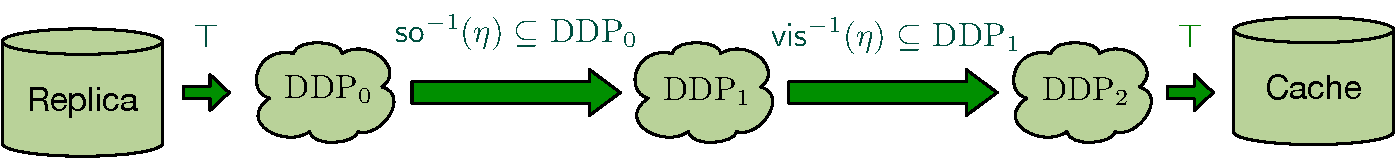
\includegraphics[scale =
	0.4]{Figures/Availability_deg.pdf}
	%}
	\\ 
	\hrulefill
\caption{Example of stepwise progress of effects before entering the
cache}
\label{fig:avail_deg}
\end{figure}

\end{comment}


%================================ SECTION SEVEN: Evaluation
\newpage
\section{Evaluation}
\label{sec:eval}
%
\begin{figure}[b]
\centering
\begin{center}
\begin{scriptsize}
\begin{tabular}{|l |  l | l|} 
\hline
 \multicolumn{1}{|c}  {\bf Benchmark} & \multicolumn{1}{c} {\bf
 Consistency} & \multicolumn{1}{c|}  {\bf
 Description}\\ [0.5ex] 
\hline
Counter  & MR & {Monotonicly increasing counter, e.g.
YouTubes' watch 
count}\\ \hline
DynamoDB  & RMW & {Integer register allowing various conditional puts and gets} \\ \hline
Online Store & RMW &  {Online store with shopping carts
and modifiable item prices} \\ \hline
Bankaccount  & 2VIS $\wedge$ RMW & {Offering deposit, withdraw and get balance operations}\\ \hline
Shopping List   &  MW $\wedge$ RMW & {A shopping list with
concurrent adds and deletes functionality}\\ \hline 
Microblog  &  MW, RMW & {A Twitter-like application modeled after
Twissandra}\\\hline
Rubis  & RMW, RMW$\wedge$2VIS & {eBay-like
application with browsing, supporting user wallet} \\
\hline
\end{tabular}
\end{scriptsize}
\end{center}
\caption{Fine-grained consistency requirement in benchmark programs}
\label{fig:dist_table}
\end{figure}

%intro: benchmark programs
In this section we present an evaluation study of our implementation,
including a report on
benchmark applications that utilize fine-grained weak consistency
requirements, expressable
in our specification language.
Fig.~\ref{fig:dist_table} presents seven of such programs, including
individual data types as well as larger programs consisted of multiple
data types. 

%multiple consistency levels for each program
Each program offers various operations, each of which is assigned a
potentially different consistency requirement,
representing the need for a multi-consistnet environement for
efficient execution of the programs. Surprisingly, we found no program
requiring causal consistency; all known consistency anomalies that operations
may be involved in, are expressable with simple contracts made of
dependency relations of length 1 or 2,
which differs from what was knwon in the context before, where all such
operations were considered to require CC.

%conjunction of consistency requirements for even a single operation
Additionally, in many cases we found operations that are involved in
multiple anomalies, requiring simultaneous enforcement of different
consistency guarantees, which shows the unfeasability of hand-writing
such guarantees, considering the vast set  of known consistency
anomalies. 
%
%example
For example, consider the bank account application, which offers
\dRV{}, \wdRV{} and \gbRV{} operations, where a \wdRV{} is a
strongly consistent operation that succeeds only if there are sufficient
funds in the account. There are two annomalies associate with
\gbRV{} in this program:
\begin{enumerate*}[label=(\roman*)]
\item when a users performs a \dRV{}, which is however, not refleceted
in the subsequent \gbRV{}
\item when a \gbRV{} witnesses a \wdRV{} effect, without witnessing all
the \dRV{} effects that were visible to it,
which may result in \gbRV{} returning a
negative balance.
\end{enumerate*}
As it is presented in Fig.~\ref{fig:dist_table}, in order to preempt
these anomalies, \gbRV{} requires
both \rmwCTRT{} and \visCTRT{} guarantees.
\begin{figure}[t]
        \centering
	\begin{subfigure}[t]{0.25\textwidth}
	\centering
	\hspace{-13mm}
	
\includegraphics[scale=0.22]{Figures/latency.pdf}
	\subcaption*{ \hspace{-10mm} (a) Latency}
	\end{subfigure}
	\begin{subfigure}[t]{0.36\textwidth}
	\centering
	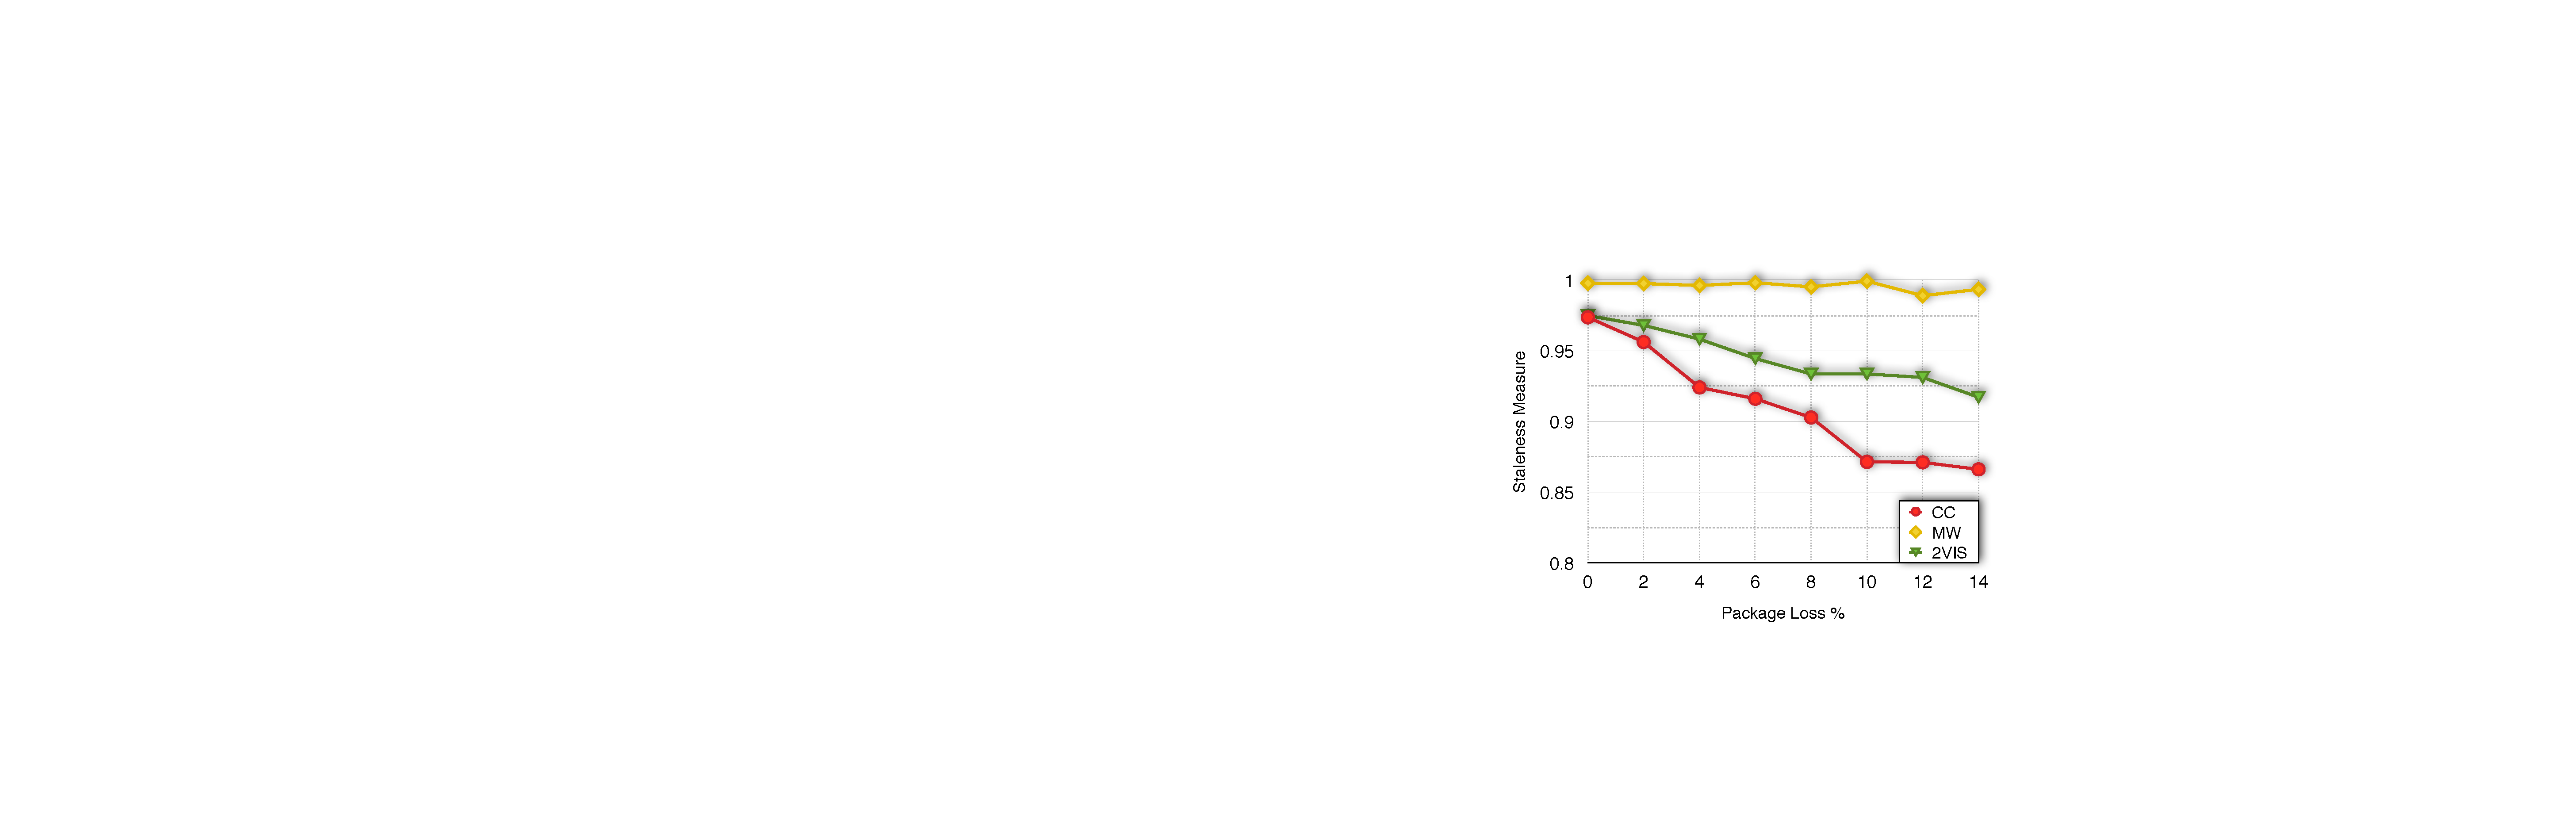
\includegraphics[scale=0.22]{Figures/staleness.pdf}
	\subcaption*{ \hspace{-1mm} (b) Staleness}
	\label{subfig:comment_example}
	\end{subfigure} 
	\begin{subfigure}[t]{0.28\textwidth}
	\centering
	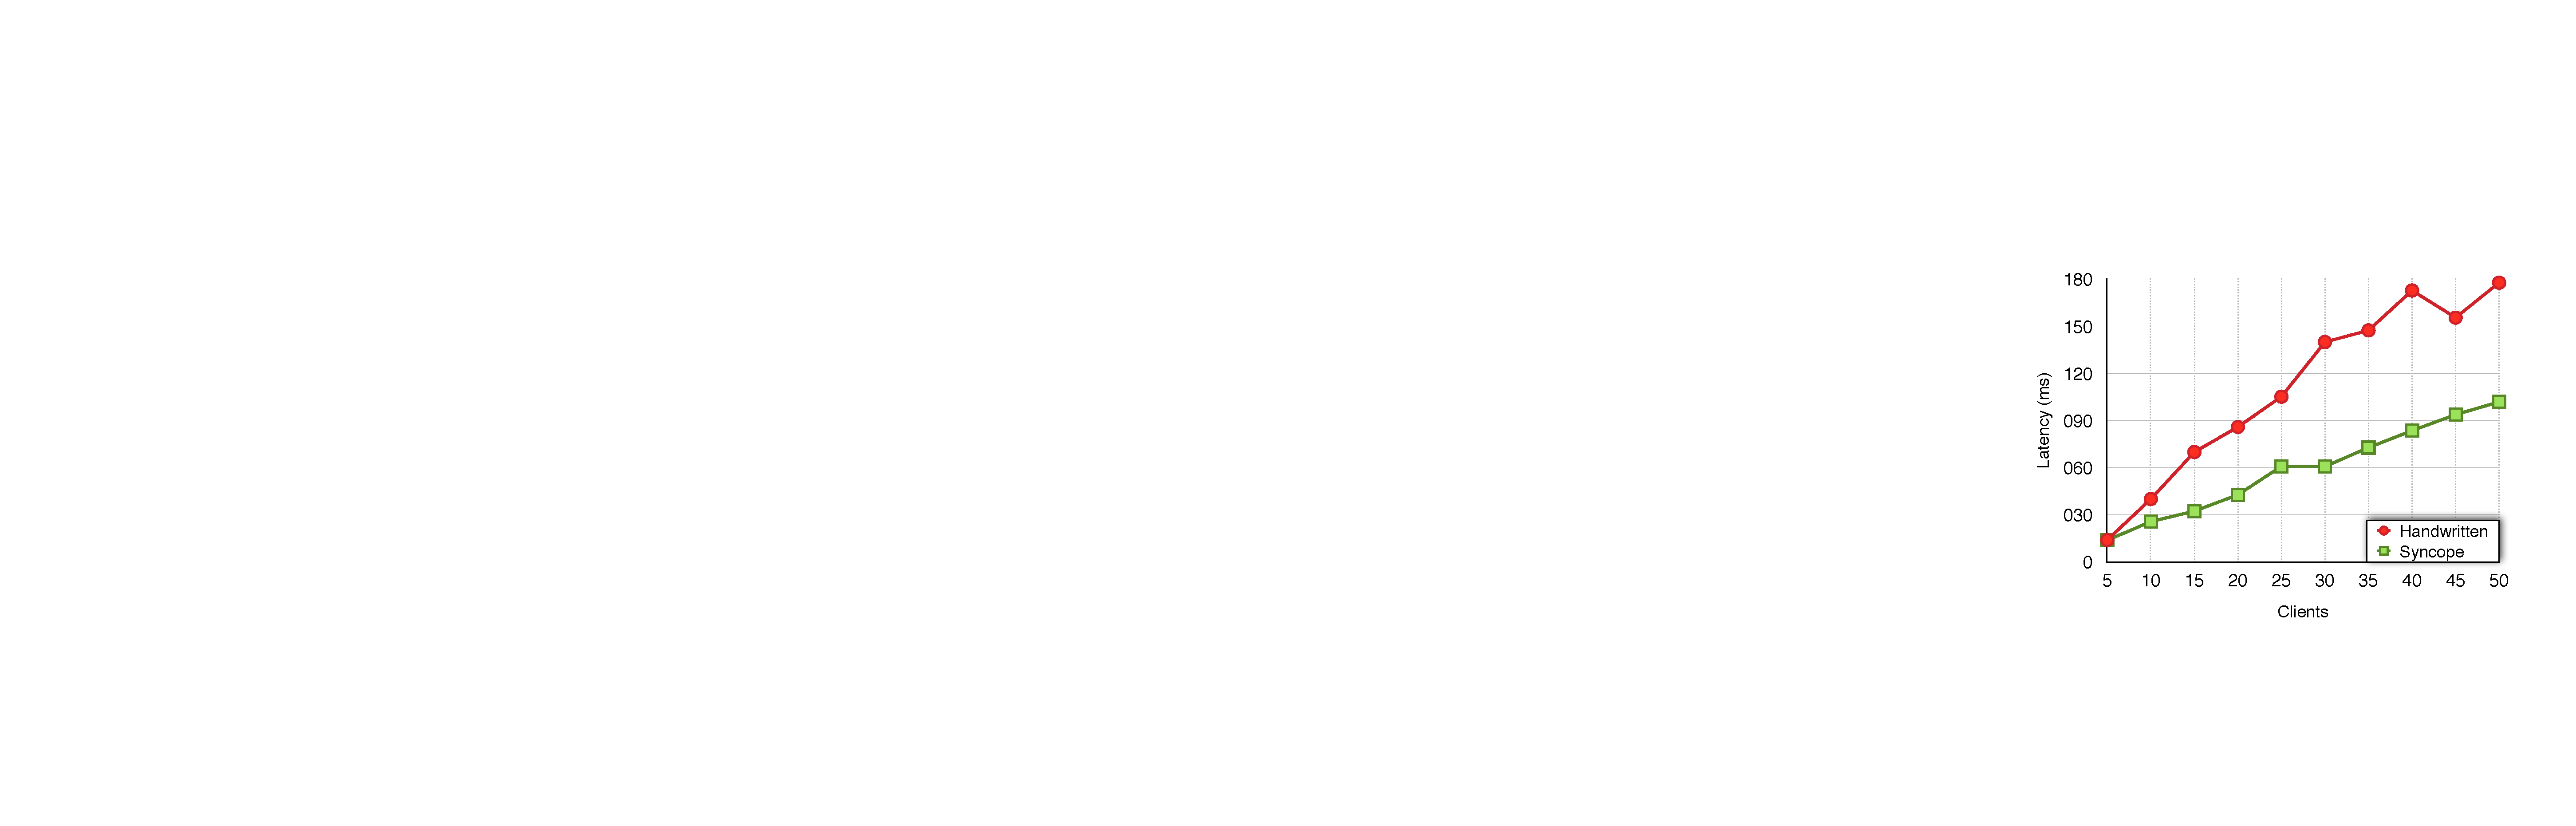
\includegraphics[scale=0.22]{Figures/comparison.pdf}
	\subcaption*{ \hspace{8mm} (c) Manual RMW}
	\label{subfig:comment_example}
	\end{subfigure} 
\\ \hrulefill
\caption{A distributed application for comment section
management}
\label{fig:eval}
\end{figure}



% performance evaluation
To evaluate its performance, we deploy \tool on a cloud cluster,
consisting of three fully replicated Cassandra replicas, running on
seperate machines within the same
datacenter. 
Each machine is instantiated with a
\tool shim layer, that responds to clients,  
 which are instantiated on a virtual machine 
co-located with one of the replicas on a machine.
We deploy the cluster on three \texttt{m4.4xlarge} Amazon EC2 instances
in US-West (Oregon) region, with inter-machine communication time of 5ms.

% The problem with Cassandra
Since Cassandra is developed over TCP connections for replica communications, 
we found all messages being  delivered with no loss and in order, making
it much more consistent  than  EC, and masking out the
differences between our fine-grained consistency guarantees.
Consequently, to simulate a
realistic EC environment, we inject random message losses at the shim
layers, where a message delivery is delayed for 1
second in case it is lost.

%The latency and staleness gain using fine-grained consistency
Fig.~\ref{fig:eval}(a) and \ref{fig:eval}(b) represent
our experimental results, with a workload generated 
by 50 concurrent clients repeatedly running sessions, each composed of three
operations, where operations uniformly choose from 5 objects and are
performed under the specified consistency level. 
We increased the
percentage of delayed messages from 0 to 14, and each experiment ran for
100 repeaded sessions per client, where the staleness measure is the
the ratio of the number of visible effects, 
to all available effects, averaged on all operations at all
replicas.

The first set of experiments, measures the client perceived latency for
three different \LB{} contracts all implemented in \tool. As expected,
causal consistency, the strongest consistency level our tool can
enforce,  experiences the larges increase in latency. The results show
$17\%$ and $67\%$ increase in latency between (RMW-MR) and (MR-CC) at only
$4$ percent message loss. These numbers go up to respectively $18\%$ and
$87\%$ at $10$ percent message loss.


















































%================================ SECTION EIGHT: Related works 
\section{Related Works}
\label{sec:rel_works}


%================================ SECTION NINE: Conclusion
\section{Conclusion}
\label{sec:conclusion}


%
% ---- Bibliography ----
%
\nocite{*}
\bibliographystyle{unsrt}
\bibliography{ref}


%% Appendix
\newpage
\appendix
\section{Modified Haskell Program}
\begin{figure}[t]
	\centering
	\begin{subfigure}[t]{0.5\textwidth}
	\begin{lstlisting}
data Sess = Bob | Alice
type ID = (Sess,Int) 
type Effect= (ID,String)
type State = (String,Int,Int)
	
read :: ID -> State -> String
read (sess,seq) (st,sq1,sq2) = 
	case sess (*@\textcolor{blue}{of}@*) 
		Bob ->   if (seq==sq1+1) (*@\textcolor{blue}{then}@*) st
		         else read (sess,seq)(st,sq1,sq2)
		Alice -> if (seq==sq2+1) (*@\textcolor{blue}{then}@*) st
		         else read (sess,seq)(st,sq1,sq2)
	\end{lstlisting}		  
	\end{subfigure}
	%
	\hfill
        %
	\begin{subfigure}[t]{0.42\textwidth}
	\begin{lstlisting}[firstnumber=13]
	apply :: State -> Effect -> State 
	apply (st,sq1,sq2) ((sess,seq),cm) = 
	  case sess (*@\textcolor{blue}{of}@*) 
	    Bob ->   if (sq1==seq-1)
	             (*@\textcolor{blue}{then}@*) (st++cm,sq1+1,sq2)
	             else (st,sq1,sq2)
	    Alice -> if (sq2==seq-1)
	             (*@\textcolor{blue}{then}@*) (st++cm,sq1,sq2+1)
	             else (st,sq1,sq2)
	\end{lstlisting}		  
        \end{subfigure}

	\hrulefill
	\caption{Guarded Application to Prevent Lost-updates Anomaly
	When Serving Bob and Alice}
	\label{fig:modified_code}
\end{figure}




\label{appendix:app}

\section{Proofs}
\label{appendix:proofs}
Here, we present the detailed proofs of the theorems of the paper. 
Let's first present a useful lemma:
\begin{lemma}
For all relations $R$ and execution steps:
\begin{fmathpar}
(\E,op_{<s,i>}) \;\xrightarrow{V}\; (\E',\eff)
\end{fmathpar}
interpretatin of $R$ under $E$ and $E'$ only differs considering $\eta$,
i.e.  {\scriptsize $a,b\not= \eta \Rightarrow (R'(a,b) \Leftrightarrow
R(a,b))$}
\label{lemma1}
\end{lemma}
\begin{proof}
We only prove $\Rightarrow$, the other part can be done
similarly. We have the following goal and hypotheses: 
\begin{fmathpar}
\begin{array}{ll}
H_0: & (\E,op_{<s,i>}) \;\xrightarrow{V}\; (\E',\eff) \\
H_1: & a,b \not= \eta\\ 
H_2: & R' (a,b)\\
G_0: & R (a,b)
\end{array}
\end{fmathpar}
Now by destructing $R$ we have the followings from new hypothesis and
goal:
\begin{fmathpar}
\begin{array}{ll}
H_3: & (\trunc{R};r)' (a,b) \\
G_1: & (\trunc{R};r) (a,b)
\end{array}
\end{fmathpar}
which can be rewritten by the definition to  get that y exists s.t.
\begin{fmathpar}
\begin{array}{ll}
H_4: & (\trunc{R})'(a,y)\\
H_5: & r'(y,b) \\
G_1: & \exists x. (\trunc{R})(a,x) \wedge (r)(x,b)
\end{array}
\end{fmathpar}
Now we instantiate the goal with y itself and by using induction on the
length of R, the first conjunct is proved, and we are left with the
following:
\begin{fmathpar}
\begin{array}{ll}
H_6: & r'(y,b) \\
G_1: & r (y,b)
\end{array}
\end{fmathpar}
Now by inversion on $H_0$ we get two cases, at both of which the
following can be derived. (In one case V should be replaced by V' but
has no effect on the proof):
\begin{fmathpar}
\begin{array}{ll}
H_7: & \visZ' = \visZ \cup V \times \{\eta\} \\
H_8: & \soZ' = \soZ' = \soZ \cup \{(\eta',\eta) \,|\, \eta'\in \EffSoup_{({\sf
SessID}=s)} 
\end{array}
\end{fmathpar}
Now, because of $H_1$ (and the fact that $y\not= \eta$) it is easy to get the following from $H_7$ and
$H_8$:
\begin{fmathpar}
\begin{array}{ll}
H_9: & \visZ(y,b) \Rightarrow \visZ(y,b) = \\
H_{10}: & \soZ(y,b) \Rightarrow \soZ(y,b) =
\end{array}
\end{fmathpar}
Which directly prove the goal, after destructing $r$.
\end{proof}








\subsection{Proof of Theorem \ref{theorem:one}}
\label{app:proof1}
\begin{footnotesize}
{\bf (Part i)}
\rule{\textwidth}{1pt}\\ \vspace{0mm} \\
 We have the following two hypotheses and the goal:
\begin{fmathpar}
\begin{array}{ll}
H_0: & (\E,op_{<s,i>}) \;\xrightarrow{V}\; (\E',\eff)  
\\
H_1: & V \; \mathtt{ is }\; \psi\mathtt{-consistent \; under \; \E} \\
G_0: & V \cup \{\eta\} \; \mathtt{is} \; \psi\mathtt{-consistent \;
under \; \E'}
\end{array}
\end{fmathpar}
Rewriting the definition in $G_0$ results in the following. We denote
the interpretation of $R$ under $E'$ as $R'$:
\begin{fmathpar}
\begin{array}{ll}
G_1: & \forall (b\in V\cup \{\eta\}).\forall (a \in E'.A). R'(a,b)
\Rightarrow a \in V \cup \{\eta\}
\end{array}
\end{fmathpar}
By intros we have: 
\begin{fmathpar}
\begin{array}{ll}
H_2: & b \in V \cup \{\eta\} \\
H_3: & a \in E'.A \\
H_4: & R' (a,b)\\
G_2: & a \in V \cup \{\eta\}
\end{array}
\end{fmathpar}
by inversion on $H_0$, there is two cases, in case \rulelabel{ub
exec} we
have the 
following:
\begin{fmathpar}
\begin{array}{ll}
T_1: &  \auxred{V'} {(\E,op_{<s,i>})} {} {(\E',\eff)}\
\end{array}
\end{fmathpar}
by inversion on $T_1$ we will have the following:
\begin{fmathpar}
\begin{array}{ll}
T_2: & E'.A = E.A \cup \{\eta\}
\end{array}
\end{fmathpar}
Since the other case (\rulelabel{lb exec}) also includes similar premises which
yields $T_2$, we can add it to the hypotheses:
\begin{fmathpar}
\begin{array}{ll}
H_5: & E'.A = E.A \cup \{\eta\}
\end{array}
\end{fmathpar}
by rewriting $H_5$ in $H_3$  and by inversion, we get two cases:
$(a=\eta)$ and $(a \in E.A)$. The first case immediatly proves $G_2$, so we
only consider the second case where we have: 
\begin{fmathpar}
\begin{array}{ll}
H_6: & a \in E.A
\end{array}
\end{fmathpar}
Now, by inversion on $H_2$, we have two cases: 
\begin{itemize}
\item {\bf Case 1:} \\
\begin{fmathpar}
\begin{array}{ll}
& b \in V 
\end{array}
\end{fmathpar}
by inversion in $H_1$ we have:
\begin{fmathpar}
\begin{array}{ll}
H_7: & \forall (x \in V). \forall (y \in E.A). R(y,x) \Rightarrow y \in
V
\end{array}
\end{fmathpar}
and by instantiating it with a and b: 
\begin{fmathpar}
\begin{array}{ll}
H_8: & R(a,b) \Rightarrow a \in V
\end{array}
\end{fmathpar}
Now by applying the lemma 1 on $H_4$ we get that $R(a,b)$ holds (since
$a,b \neq \eta$), which can be applied on $H_8$ to get $a \in V$ which
proves the goal $G_2$.
\vspace{3mm}
%
%
%
%
\item {\bf Case 2:} \\
\begin{fmathpar}
\begin{array}{lll}
& H_9: & b = \eta \\
\hspace{-35 mm} \mathtt{(by \; rewriting \;} H_9 \mathtt{\;in\; } H_4) & H_{10}: & R'(a,\eta)
\end{array}
\end{fmathpar}
Now we use inversion on $H_0$ and get two cases: \rulelabel{LB exec} and
\rulelabel {UB exec}:
\subitem {\bf \footnotesize SCase \rulelabel{LB exec}}:
we have $H_{11}$ and $H_{12}$ from the reduction rule premises:
\begin{fmathpar}
\begin{array}{ll}
H_{11}: & R^{-1}_V(\eta) = R^{-1}_{E'.A}(\eta)   \\ \vspace{-2mm}\\
H_{12}: & R_V^{-1}(\eta) \subseteq V
\end{array}
\end{fmathpar}
now from $H_{10}$ we have $H_{13}$ which can be rewritten by $H_{11}$ to
get $H_{H14}$:
\begin{fmathpar}
\begin{array}{ll}
H_{13}: & a \in R^{-1}_{E'.A}(\eta)\\
H_{14}: & a \in R^{-1}_{V}(\eta)
\end{array}
\end{fmathpar}
The goal $G_2$ is now proved from $H_{12}$ and $H_{14}$.

\subitem {\bf \footnotesize SCase \rulelabel{UB exec}}:
We have the following from the premises: 
\begin{fmathpar}
\begin{array}{ll}
H_{15}: & V' = \left \lfloor V  \right \rfloor_{\mathtt{max}}\\
H_{16}: & V' \subseteq V
\end{array}
\end{fmathpar}
By destructing $R$, the only non-trivial cases are
$(R=\trunc{R};\visZ)$ and 
($R=\visZ$):


{\bf SSCase }($R=\trunc{R};\visZ$):  \\
From $H_{10}$ we get $H_{17}$ which based on the definition, yields that
there exists $c$ such that $H_{18}$, $H_{19}$ and $H_{20}$ hold:
\begin{fmathpar}
\begin{array}{ll}
H_{17}: & a \in (\trunc{R}';\visZ')_{E'.A}^{-1}(\eta)\\
H_{18}: & c \in \visZ'^{-1}(\eta)\\
H_{19}: & a \in \trunc{R}'^{-1}(c)\\
H_{20}: & \visZ'^{-1}(\eta) \subseteq E'.A \\
\end{array}
\end{fmathpar}
from $H_{15}$ we have:
\begin{fmathpar}
\begin{array}{ll}
H_{21}: & (\trunc{R})^{-1}_V(V') \subseteq V'
\end{array}
\end{fmathpar}
Now from $H_{18}$ (and $T_1$) it is straightforward to get:
\begin{fmathpar}
\begin{array}{ll}
H_{22}: & c \in V'
\end{array}
\end{fmathpar}
which after appying the lemma 1 on $H_{19}$, and by $H_{21}$ yields the following, which proves
the goal $G_2$:
\begin{fmathpar}
\begin{array}{ll}
H_{23}: & a \in V'
\end{array}
\end{fmathpar}

{\bf SSCase }($R=\visZ$): 
From $H_{10}$ we get that $\visZ' (a,\eta)$, which -with a similar
argument to the previous subcase- yields the following and the goal is
proved: 
\begin{fmathpar}
\begin{array}{ll}
H_{24}: & a \in V'
\end{array}
\end{fmathpar}
\end{itemize} 
\fcolorbox{red}{white}{\color{black} \footnotesize QED.}  \vspace {10mm} \\ 
%
%
%
%
%
%
%
{\bf (Part ii)}  
\rule{\textwidth}{1pt}\\ \vspace{0mm} \\
For this part we have the  following hypothesis and the goal:
\begin{fmathpar}
\begin{array}{ll}
H_{0}: & (\E,op_{<s,i>}) \;\xrightarrow{V}\; (\E',\eff) \\ 
G_{0}: & E' \models [\eta/\hat{\eta}]
\end{array}
\end{fmathpar}
By inversion on $H_0$, we have two cases: \\
{\footnotesize \bf Case1} \rulelabel {UB exec}:\\
\begin{fmathpar}
\begin{array}{ll}
H_{1}: & r_k = \visZ\\ 
H_{2}: & V \subseteq E.A \\
H_{3}: & V'= \left \lfloor V  \right \rfloor_{\mathtt{max}}\\
H_{4}: & \auxred{V'} {(\E,op_{<s,i>})} {} {(\E',\eff)}\\
\end{array}
\end{fmathpar}
The goal $G_0$ can also be rewritten as: 
\begin{fmathpar}
\begin{array}{ll}
G_{1}: & E' \models \forall a. a \xrightarrow{R} \eta \Rightarrow a
\xrightarrow{vis} \eta 
\end{array}
\end{fmathpar}
Since the $E'.A$ gives the interpretation for the universe of
quantification:
\begin{fmathpar}
\begin{array}{ll}
G_{2}: & \forall (a\in E'.A). E' \models a \xrightarrow{R} \eta \Rightarrow a
\xrightarrow{vis} \eta 
\end{array}
\end{fmathpar}
by intros: 
\begin{fmathpar}
\begin{array}{ll}
H_{5}: & a \in E'.A\\
G_{3}: & E' \models a \xrightarrow{R} \eta \Rightarrow a
\xrightarrow{vis} \eta 
\end{array}
\end{fmathpar}
Now since ({\scriptsize $(\mathcal{M} \models A \Rightarrow B) \Leftrightarrow
(\mathcal{M} \models A   \Rightarrow  \mathcal{M} \models B)$}) we can rewrite $G_3$ as:
\begin{fmathpar}
\begin{array}{ll}
G_{4}: & (E' \models a \xrightarrow{R} \eta) \Rightarrow (E' \models a
\xrightarrow{vis} \eta) 
\end{array}
\end{fmathpar}
by intros: 
\begin{fmathpar}
\begin{array}{ll}
H_{6}: & E' \models a \xrightarrow{R} \eta \\
G_{5}: & E' \models a \xrightarrow{vis} \eta 
\end{array}
\end{fmathpar}
Now we use the interpretation given by $E'$, to rewrite the relations as
follows. Note that we denote the interpretation of $R$ under $E'$ as
$R'$ and $E.\visZ$ as $\visZ'$.
\begin{fmathpar}
\begin{array}{ll}
H_{7}: & R'(a,\eta) \\
G_{6}: & \visZ'(a,\eta)
\end{array}
\end{fmathpar}
by inversion on $H_4$:
\begin{fmathpar}
\begin{array}{ll}
H_{8}: & \visZ' = \visZ \cup V' \times \{\eta\}
\end{array}
\end{fmathpar}
Now since $\eta\not\in E.A$, we get that $a \in V' \Rightarrow
\visZ'(a,\eta)$, which can be applied to $G_6$ to get the following:
\begin{fmathpar}
\begin{array}{ll}
G_{7}: & a \in V'
\end{array}
\end{fmathpar}
Now, destructing R yileds multiple cases, only one of which is
non-trivial:  
$\scriptsize R=\trunc{R};\visZ$, which can be rewritten in $H_7$ to get:
\begin{fmathpar}
\begin{array}{ll}
H_{9}: & (\trunc{R};\visZ)'(a,\eta)
\end{array}
\end{fmathpar}
Now we can rewrite the definition in $H_9$, and derive that there exists
$b$ such that:
\begin{fmathpar}
\begin{array}{ll}
H_{10}: & \trunc{R}'(a,b)\\
H_{11}: & \visZ'(b,\eta)\\
\end{array}
\end{fmathpar}
Now using a similar argument, from $H_8$ and $H_{11}$ we get: 
\begin{fmathpar}
\begin{array}{ll}
H_{12}: & b \in V'\\
\end{array}
\end{fmathpar}
Now by applying the lemma 1 on $H_{10}$ we get: 
\begin{fmathpar}
\begin{array}{ll}
H_{13}: & \trunc{R}(a,b)
\end{array}
\end{fmathpar}
since we have {\scriptsize $V' \in \left \lfloor V  \right \rfloor$}, 
we get the following: 
\begin{fmathpar}
\begin{array}{ll}
H_{14}: & \forall (x\in V'). (\trunc{R})_{E.A}^{-1}(V') \Rightarrow x \in V'
\end{array}
\end{fmathpar}
which yields the following from $H_{12}$ and $H_{13}$:
\begin{fmathpar}
\begin{array}{ll}
H_{15}: & a \in V'
\end{array}
\end{fmathpar}
which proves the goal $G_7$.\\ \vspace{3 mm} \\
{\footnotesize \bf Case2} \rulelabel{LB exec}:\\
We prove this case by induction on the length of the given relation $R$.
We have the followings, from the premises of the reduction rule:
\begin{fmathpar}
\begin{array}{ll}
H_{1}: & r_k = \soZ\\ 
H_{2}: & V \subseteq E.A \\
H_{3}: & R^{-1}_V(\eta) = R^{-1}_{E.A}(\eta)\\
H_{4}: & R^{-1}_V(\eta) \subseteq V \\
H_{5}: & \auxred{V} {(\E,op_{<s,i>})} {} {(\E',\eff)}\\
\end{array}
\end{fmathpar}
Using the same argument as the previous section, we get the following
new goal and hypotheses:
\begin{fmathpar}
\begin{array}{ll}
H_{6}: & a \in E'.A\\ 
H_{7}: & R'(a,\eta) \\
G_{1}: & \visZ'(a,\eta)
\end{array}
\end{fmathpar}
We now destruct R to get $H_8$ from $H_7$, and rewrite the definition in it to get the next
two hypotheses.
Note that by destructing $R$, there are only two non-trivial cases
$(R=\trunc{R};\soZ)$ and $(R=\soZ)$, which we only consider the
former, since the latter can be proved similarly:
\begin{fmathpar}
\begin{array}{ll}
H_{8}: & (\trunc{R};\soZ)'(a,\eta) \\ 
H_{9}: & \trunc{R}'(a,b)\\
H_{10}: & \soZ'(b,\eta)
\end{array}
\end{fmathpar}
Now, from the previous section we know that $(so')^{-1}(\eta) \subseteq V$
which yields the following from $H_{10}$:
\begin{fmathpar}
\begin{array}{ll}
H_{11}: & b \in V
\end{array}
\end{fmathpar}
The goal is proved by the induction hypothesis, $H_9$ and $H_{11}$.
\\ \fcolorbox{red}{white}{\color{black} \footnotesize QED.}
\end{footnotesize}
\\
























\subsection{Proof of Theorem \ref{theorem:two}}
\label{app:proof2}
By contradiction:
\begin{smathpar}
\begin{array}{ll}
H_0: & (\E,op_{<s,i>}) \;\xrightarrow{V}\; (\E',\eff)\\
H_1: & (\E,op_{<s,i>}) \;\xrightarrow{V}\; (\E'',\eff)\\
H_2: & a \in   (E''.vis^{-1}(\eta)) \\
H_3: & a \not\in  (E'.vis^{-1}(\eta))\\
G_0: & \bot 
\end{array}
\end{smathpar}
By inversion on $H_1$ we have: 
\begin{smathpar}
\hspace{-48 mm}
\begin{array}{lcl}
&H_4: & \auxred{V''} {(\E,op_{<s,i>})} {} {(\E'',\eff)}\\
&H_5: &   V''= \left \lfloor V \right \rfloor_V \\
(\mathtt{by \;inversion \;on\;} H_4 \mathtt{\;and \;from\;} H_2) & H_6: & a \in V''
\end{array}
\end{smathpar}
By inversion on $H_0$ and following a similar argument we can now derive: 
\begin{smathpar}
\begin{array}{ll}
H_7: &  \auxred{V''} {(\E,op_{<s,i>})} {} {(\E',\eff)} \\
H_8: & V'= \left \lfloor V \right \rfloor_V \\
H_9: & a \not\in V'\\
\end{array}
\end{smathpar}
However from $H_5$ we know $V''\subseteq V \wedge R_V^{-1}(V'')\subseteq V''$, which results in contradiction because of the maximality of $V'$ defined in $H_8$.


\subsection{Proof of Theorem \ref{theorem:three}}
\label{app:proof3}
\begin{footnotesize}
Before proving the theorem, we first present and prove a useful lemma
and then we will present 
a new definition, regarding sets of effects.
\vspace{2mm}
\hrule
\begin{lemma}
Under an execution state E and for a given set $S \subseteq E.A$, if
$S$ is $\psi$-consistent under $E$, then $\forall(x\in S).R_S^{-1}(x)
\subseteq S$ under $E$.
\end{lemma}
\begin{proof}
\begin{fmathpar}
\begin{array}{ll}
H_0: & S is \psi\mathtt{-consistent} \\
G_0: & \forall(x\in S). R_{S}^{-1}(x) \subseteq S \\
\end{array}
\end{fmathpar}
after intros:
\begin{fmathpar}
\begin{array}{ll}
H_1: & x \in S\\
G_1: & R_{S}^{-1}(x) \subseteq S \\
\end{array}
\end{fmathpar}
inversion on $H_0$ gives the following:
\begin{fmathpar}
\begin{array}{ll}
H_2: & \forall (\eta \in S).\forall(a\in E.A). R(a,\eta) \Rightarrow a
\in S \\
\end{array}
\end{fmathpar}
which can be rewritten to:
\begin{fmathpar}
\begin{array}{ll}
H_3: & \forall (\eta \in S). R^{-1}(\eta) \subseteq S\\
\end{array}
\end{fmathpar}
however, since $S\subseteq E.A$ then\footnote{\scriptsize we skip the formal proof
of this claim, however, since the only difference in the definitions of
$R^{-1}$ and $R^{-1}_S$ is the extra requirement about mid-level
effects in the latter, it should be a subset of the former.}:
\begin{fmathpar}
\begin{array}{ll}
H_4: & \forall (a\in E.A).R^{-1}_S(a) \subseteq R^{-1}(a)  \\
\end{array}
\end{fmathpar}
Now we can instantiate $H_3$ and $H_4$ into:
\begin{fmathpar}
\begin{array}{ll}
H_5: & R^{-1}(x) \subseteq S \\
H_6: & R^{-1}_S(x) \subseteq R^{-1}(x) 
\end{array}
\end{fmathpar}
which trivially yields $G_1$ and the proof is completed.\\
\fcolorbox{red}{white}{\color{black} \footnotesize QED.}
\vspace{2mm}
\hrule
\end{proof}
\label {lemma1}
\end{footnotesize}
\begin{footnotesize}
\begin{definition} 
We define the completment of a given set of effects $S$ (under an
execution state $E$) as the super set of $S$, containing ALL the
mid-level effects required to determine ALL the dependencies of the
effects in $S$, i.e.
\begin{fmathpar}
\begin{array}{lll}
S' \in  \left \lceil S \right \rceil \iff  R^{-1}_{S'}(S) = R^{-1}_{E.A}(S)
\end{array}
\end{fmathpar}
\end{definition}

Now, using the above theorem and lemma, we present the proof of the
theorem 3, which starts by listing the following hypotheses and the goal:
\begin{fmathpar}
\begin{array}{ll}
H_0: & \auxred{S} {(\E,op_{<s,i>})} {} {(\E',\eff)}    \\
H_1: & S \cup \{\eta\} \; is \;  \psi\mathtt{-consistent}\\
G_0: & \exists E''.\exists \eta'. \exists V.
((\E,op_{<s,i>})\;\xrightarrow{V}\;(\E'',\eff'))
\end{array}
\end{fmathpar}
Now, by destructing $R$ we get two non-trivial cases:
\begin{itemize}
\item {\bf Case1}($R=\trunc R ;\visZ$):\\
In this case, we generate the premises of the \rulelabel{ub exec} to
achieve the goal. We define the following: 
\begin{fmathpar}
\begin{array}{ll}
H_3: & S' = \left
\lfloor S \right \rfloor_{\mathtt{max}} \\\vspace{1mm}
H_4: & \eta' = F_{op}(S')
\end{array}
\end{fmathpar}




\begin{fmathpar}
\begin{array}{ll}
H_2: & V = S\\
G_1: & \exists E''.\exists \eta'.
((\E,op_{<s,i>})\;\xrightarrow{S}\;(\E'',\eff'))
\end{array}
\end{fmathpar}








\item {\bf Case2}($R=\trunc R;\soZ$):\\
\end{itemize}










\end{footnotesize}




\newpage
\section{Operational Semantics of the Augmented algorithm}
\label{appendix:large_semantics}
Here, we explain our detailed operational semantics, to maintain
multi-consistent replicated stores. We assume a given function from
operation names, to consistency contracts: $\Psi :  op \mapsto \psi $
and for simplicity reasons (again, it can be easily generalized) we
consider contracts made by a single prop:
\begin{smathpar}
\Psi(op)=\forall (a,b). a \xrightarrow{R_{op}} \Rightarrow a \xrightarrow{vis} b. 
\end{smathpar}
For a given realtion $R$ we also define $R[m]$ to refer to the m'th
relation seed in $R$:
\begin{smathpar}
(r_1;r_2;...;r_m;...;r_k)[m] = r_m
\end{smathpar}


In this section we introduce the complete behavior of our multi-consistenct shim layer as a new set of operational semantics. 
The rules are parametrized over a given map of operation names to
contracts, $\Psi :  op
\mapsto \psi $ and we assume each contract is of the form:
$\Psi(op)=\forall (a,b). a \xrightarrow{Q_{op}} \Rightarrow a \xrightarrow{vis} b.$ 
We use $Q_{op}[m]$ notation to refer to the m'th clause in the composition.
We define a pool to be a set of effects and a value that contains all
the effects that arrive to the replica. 
Our shim layer, also maintains a set of k caches (one cache for each
given contract). Each cache is maintained to be the largest
subset of pool that is closed under its
contract.  i.e. $\forall \eff \in \Cache(op). Q_{op}^{-1}(\eff)
\subseteq \Cache(op) $ 
\\We also maintain a level of availability for each effect
according to an operation and the current pool. If the availability of an effect for
$op$ is $x$, it means
that the effect satisfies the suffix of size $x$ of contract $\Psi(op)$.
An effect $\eta$ satisfies a suffix of size $x\geq 1$ of contaract
$\psi=\forall (a,b). a \xrightarrow{q_1;q_2;...;q_n} b$,
written as $ (\eta \models_{\Pool}^{x} \psi )$, if and only if
$(q_{n-(x-1)};...;q_{n} )^{-1}_{\Pool}(\{\eta\}) \subseteq \Pool$. The
initial availability value for all effects is 0, and increases when more
dependent effects arrive. 
\\
Following are the formal definitions: 
\\
\begin{figure*}[h]
\raggedright
%

\textbf{Auxiliary Definitions}\\
%
\begin{minipage}{\columnwidth}
\begin{smathpar}
\stretcharraybig
\begin{array}{lclcl}
  \multicolumn{5}{c}{
    {\delta} \in \mathtt{Replicated\; Data\; Type} \spc\spc
    {v} \in \mathtt{Value}\spc\spc
    {op} \in \mathtt{Operation\; Name}
  }\\
  \multicolumn{5}{c}{
    {s} \in \mathtt{Session\; Id} \spc\spc
    {i} \in \mathtt{Effect\; Id} \spc\spc
    {\rho} \in \mathtt{Replica\; Id}
  }\\
  \eff & \in & \mathtt{Effect} & \coloneqq &  (s,i,op,v)\\
   {\Pool} & \in & \mathtt {Pool} & \coloneqq & (v,\set {\eff}) \\
   {\Cache} & \in & \mathtt {Cache} & \coloneqq & (v,\set{\eff})\\
  F_{op} & \in & \mathtt{Op.\,Def.} & \coloneqq & v \rightarrow \eta\\
  \EffSoup & \in & \mathtt{Eff\,Soup}	  & \coloneqq & \set{\eff} \\
  \visZ,\soZ &	\in & \mathtt{Relations} & \coloneqq & \set{(\eff,\eff)} \\
  {\E} 		& \in & \mathtt{Exec\;State}  & \coloneqq & \Exec \\
  \Theta  & \in & \mathtt{Store}      & \coloneqq & \rho \mapsto (\Pool,\Cache) \\
  {\sigma} 	& \in & \mathtt{Session} 					 	& \coloneqq & \cdot \ALT op::\sigma \\
  \Sigma 		& \in & \mathtt{Session\;Soup}   	 	& \coloneqq &
        \langle s, i, \sigma \rangle \pll \Sigma \ALT \emptyset \\
\end{array}
\end{smathpar}
\end{minipage}
%

\begin{smathpar}
\begin{array}{c}
\ssn(s,\_,\_,\_) = s \spc\spc
\id(\_,j,\_,\_) = j \spc\spc
\oper(\_,\_,op,\_) = op \spc\spc
\rval(\_,\_,\_,n) = n\\
\end{array}
\end{smathpar}

\vspace{5mm}
\textbf{Auxiliary Reduction} \;
  \fbox{\(\auxred{v} {(\E,\langle s,i,op \rangle)} {} {(\E',\eff)}\)}\\

\begin{minipage}{\textwidth}
\rulelabel{Oper}
\begin{smathpar}
\stretcharraybig
\begin{array}{l}
\RuleTwo
{
%\Theta(\rho \mapsto (v,cache)) \qquad
F_{op}(v) = \eta \qquad
\ssn(\eta) = s \qquad 
\id(\eta) = i \qquad
%\{\eff'\} = \EffSoup_{({\sf SessID}=s,\,{\sf SeqNo}=i-1)}\\
\EffSoup' = \EffSoup \cup \{\eff\} \\
\visZ' = \visZ \cup S \times\{\eff\}\qquad
\soZ' = \soZ \cup \{(\eta',\eta) \,|\, \eta'\in \EffSoup \conj 
    \ssn(\eta')=s \conj \id(\eta')<i\}\qquad
%\soZ' = (\soZ^{-1}(\eff') \cup \eff') \times\{\eff\} \cup \soZ
}
{
  \auxred {v} {((\EffSoup,\visZ,\soZ), \langle s,i,op \rangle}
  {} {((\EffSoup',\visZ',\soZ'),\eta)}
}
\end{array}
\end{smathpar}
\end{minipage}


\vspace{5mm}
\textbf{Operational Semantics} \;
  \fbox{\((\E,\Theta,\Sigma) \;\xrightarrow{\eff}\; (\E',\Theta',\Sigma')\)}\\

\begin{minipage}{3in}
\rulelabel{Pool Refresh}
\begin{smathpar}
\stretcharraybig
\begin{array}{l}
\RuleTwo
{ 
  \eta \in \E.\EffSoup \spc
  \Theta(\rho) = (\Pool,\Cache) \spc
  \eta \not\in \Pool_e \\
  \Pool' = (apply \; \eta\; \Pool_v,\Pool_e \cup \{\eta\}) \spc \\
  \Theta' = \Theta[\rho \mapsto (\Pool',\Cache)]\\
}
{
  (\E,\Theta,\Sigma) \;\xrightarrow{\eff}\; (\E, \Theta', \Sigma)
}
\end{array}
\end{smathpar}
\end{minipage}

\vspace{5mm}
\begin{minipage}{2.8in}
\rulelabel{Cache Refresh}
\begin{smathpar}
\stretcharraybig
\begin{array}{l}
\RuleTwo
{
  \Theta(\rho) = (\Pool,\Cache) \spc \eta \in \Pool_e
  \\ \eta \not\in \Cache_e \spc
  \Cache'=(apply \; \eta \; \Cache_v ,\Cache_e \cup \{\eta\}) \\ \psi^{-1}
  (\eta) \subseteq \Cache_e
 \spc  \Theta' = \Theta[\rho \mapsto (\Pool,\Cache')]\\
}
{
  (\E,\Theta,\Sigma) \;\xrightarrow{\eff}\; (\E, \Theta', \Sigma)
}
\end{array}
\end{smathpar}
\end{minipage}
\hspace{12 mm}
\vspace{3mm}
\begin{minipage}{2.3in}
\rulelabel{Exec}
\begin{smathpar}
\stretcharraybig
\begin{array}{l}
\RuleTwo
{
  \auxred{\CacheFinder_{\psi}(\Theta(\rho))} {(\E,\langle s,i,op \rangle)} {} {(\E',\eta)}  \\
  \Theta(\rho) = (\Pool,\Cache) \spc \psi^{-1}(\eta) \subseteq \Pool_e  \spc
}
{
  (\E,\Theta,\langle s,i,op::\sigma \rangle \pll \Sigma) 
    \;\xrightarrow{\eff}\;
  (\E',\Theta,\langle s,i+1,\sigma \rangle \pll \Sigma) 
}
\end{array}
\end{smathpar}
\end{minipage}


\caption{Operational semantics of a replicated data store.}
\label{sem:oper}
\end{figure*}











\end{document}
